\section{ỨNG DỤNG HÌNH HỌC CỦA TÍCH PHÂN}
\subsection{Diện tích hình thang cong}
\subsubsection{Hình phẳng giới hạn bởi đồ thị hàm số, trục hoành và hai đường thẳng $x=a$ và $x=b$}
\begin{center}
	\begin{tikzpicture}[scale=1,font=\footnotesize,line join=round,line cap=round,>=stealth]
	% Draw axes
	\draw[->] (-0.5,0) -- (6,0) node[right] {$x$};
	\draw[->] (0,-0.5) -- (0,4) node[above] {$y$};
	
	% Labels
	\node at (0,0) [below left] {$O$};
	\node at (0.7,0) [below] {$a$};
	\node at (4.3,0) [below] {$b$};
	\node at (5.3,2) {$y = f(x)$};
	
	% Draw function curve
	\draw[thick,domain=0.5:4.7,samples=100] plot (\x,{-0.3*(\x-0.8)*(\x-2.5)*(\x-5)+1.5});
	
	% Draw vertical lines
	\draw[dashed] (0.7,0) -- (0.7,{-0.3*(0.7-0.8)*(0.7-2.5)*(0.7-5)+1.5});
	\draw[dashed] (4.3,0) -- (4.3,{-0.3*(4.3-0.8)*(4.3-2.5)*(4.3-5)+1.5});
	
	% Draw shaded area
	\fill[pattern=north east lines, pattern color=black!50] 
	(0.7,0) -- plot[domain=0.7:4.3,samples=100] (\x,{-0.3*(\x-0.8)*(\x-2.5)*(\x-5)+1.5}) -- (4.3,0) -- cycle;
	
	% Additional labels
	\node at (0.5,2.7) [below] {$x = a$};
	\node at (4.5,3.5) [below] {$x = b$};
	\node at (3.5,-0.1) [below left] {$y = 0$};
\end{tikzpicture}
\end{center}
Cho hàm số $y=f(x)$ liên tục trên $[a;b]$. Khi đó, diện tích hình phẳng giới hạn bởi đồ thị hàm số $y=f(x)$, trục hoành $Ox$ $(y=0)$ và hai đường thẳng $x=a$ và $x=b$ được tính bởi công thức

	$$S=\displaystyle\int\limits_a^b \left|f(x)\right|\mathrm{\,d}x$$

\textbf{Chú ý:} Giả sử hàm số $y=f(x)$ liên tục trên $[a;b]$. Nếu $f(x)$ không đổi dấu trên $[a;b]$ thì

	$$\displaystyle\int\limits_a^b \left|f(x)\right|\mathrm{\,d}x=\displaystyle\left|\int\limits_a^b f(x)\mathrm{\,d}x\right|.$$

\subsubsection{Hình phẳng giới hạn bởi hai đồ thị hàm số và hai đường thẳng $x=a$ và $x=b$}

\begin{center}
	\begin{tikzpicture}[scale=1,font=\footnotesize,line join=round,line cap=round,>=stealth]
	% Draw axes
\draw[->] (-0.5,0) -- (6,0) node[right] {$x$};
\draw[->] (0,-0.5) -- (0,4) node[above] {$y$};

% Labels
\node at (0,0) [below left] {$O$};
\node at (0.7,0) [below] {$a$};
\node at (4.3,0) [below] {$b$};
\node at (5,3.1) {$y = f(x)$};
\node at (5,2.1) {$y = g(x)$};
% Draw function curve
\draw[thick,domain=1:3.7,samples=100] plot (\x,{sqrt(4-(\x-2.5)^2)+1.5});
\draw[thick,domain=0.9:3.9,samples=100] plot (\x,{-sqrt(4-(\x-2.5)^2)+3.3});

% Draw vertical lines
\draw[dashed] (1.2,0) -- (1.2,{sqrt(4-(1.2-2.5)^2)+1.5});
\draw[dashed] (3.4,0) -- (3.4,{sqrt(4-(3.4-2.5)^2)+1.5});

% Draw shaded area
\fill[pattern=north east lines, pattern color=black!50] 
(1.2,1.78) -- plot[domain=1.2:3.4,samples=100] (\x,{sqrt(4-(\x -2.5)^2)+1.5}) -- (3.4,1.514) -- plot[domain=1.2:3.4,samples=100] (\x,{-sqrt(4-(\x-2.5)^2)+3.3}) -- cycle;

% Additional labels
\node at (1.2,4) [below] {$x = a$};
\node at (3.4,4) [below] {$x = b$};

\end{tikzpicture}
\end{center}
Cho 2 hàm số $y=f(x)$ và $y=g(x)$ liên tục trên $[a;b]$. Khi đó diện tích của hình phẳng giới hạn bởi đồ thị hai hàm số $y=f(x)$ và $y=g(x)$ và hai đường thẳng $x=a$ và $x=b$ được tính bởi công thức
$$
S=\displaystyle\int_a^b|f(x)-g(x)|\mathrm{\,d}x
$$
\subsection{Thể tích hình khối}
\subsubsection{Thể tích của vật thể}
\begin{center}
\begin{tikzpicture}[scale=1,font=\footnotesize,line join=round,line cap=round,>=stealth]
	\draw plot[smooth,tension=.65] coordinates{(1,2) (2.5,2.3) (3.5,2.2)};
	\draw[dashed] plot[smooth,tension=.65] coordinates{(3.5,2.2) (4,2)};
	\draw plot[smooth,tension=.65] coordinates{(4,2) (5,2.2) (5.5,2.1)};
	\draw[dashed] plot[smooth,tension=.65] coordinates{(5.5,2.1) (6,2)};
	\draw plot[smooth,tension=.65] coordinates{(1,1) (2.3,0.5) (3.5,0.8)};
	\draw[dashed] plot[smooth,tension=.65] coordinates{(3.5,0.8) (4,1)};
	\draw plot[smooth,tension=.65] coordinates{(4,1) (5,0.7) (5.5,0.8)};
	\draw[dashed] plot[smooth,tension=.65] coordinates{(5.5,0.8) (6,1)};
	\draw[dashed] (1,1) arc (-90:90:.2 and 0.5);
	\draw (1,2) arc (90:270:.2 and 0.5);
	\draw[dashed] (4,1) arc (-90:90:.2 and 0.5);
	\draw (4,2) arc (90:270:.2 and 0.5);
	\draw (6,1) arc (-90:270:.2 and 0.5);
	\fill[pattern=north east lines] (4,1) arc (-90:90:.2 and 0.5)--(4,2) arc (90:270:.2 and 0.5)--cycle;
	\draw (-.5,0)--(0.5,0) (1,0)--(3.5,0) (4,0)--(5.5,0);
	\draw[dashed] (0.5,0)--(1,0) (3.5,0)--(4,0) (5.5,0)--(6,0);
	\draw[->] (6,0)--(7,0)node[below]{$x$};
	\draw (0.5,-1)--(0.5,3)--(1.5,3.5)--(1.5,2.2) (1.5,.8)--(1.5,-0.5)--(0.5,-1);
	\draw[dashed](1.5,2.2)--(1.5,.8);
	\draw[dashed] (1,1)--(1,0)node[below]{$a$};
	\coordinate (A) at (0.5,3);
	\coordinate (B) at (1.5,3.5);
	\coordinate (C) at (1.5,2.2);
	%\tkzMarkAngle[size=.6](A,B,C);
	\draw pic[draw=black, angle eccentricity=1.6, angle radius=0.5cm]{angle=A--B--C};
	\draw (1.3,3.2) node {\footnotesize $P$};
	\draw (3.5,-1)--(3.5,3)--(4.5,3.5)--(4.5,2) (4.5,1)--(4.5,-0.5)--(3.5,-1);
	\draw[dashed](4.5,2)--(4.5,1);
	\draw[dashed] (4,1)--(4,0)node[below]{$x$};
	\coordinate (D) at (3.5,3);
	\coordinate (E) at (4.5,3.5);
	\coordinate (F) at (4.5,2);
	%	\tkzMarkAngle[size=.6](D,E,F);
	\draw pic[draw=black, angle eccentricity=1.6, angle radius=0.5cm]{angle=D--E--F};
	\draw (4.3,3.2) node {\footnotesize $R$};
	\draw (5.5,-1)--(5.5,3)--(6.5,3.5)--(6.5,-0.5)--(5.5,-1);
	\draw[dashed] (6,1)--(6,0)node[below]{$b$};
	\coordinate (G) at (5.5,3);
	\coordinate (H) at (6.5,3.5);
	\coordinate (K) at (6.5,-0.5);
	%	\tkzMarkAngle[size=.6](G,H,K);
	\draw pic[draw=black, angle eccentricity=1.6, angle radius=0.5cm]{angle=G--H--K};	\draw (6.3,3.2) node {\footnotesize $Q$};
	\draw (0,.3) node {$O$};
	\fill (0,0) circle(1pt);
	\draw[->] (4,1.5)--(4.7,1.7) node[right] {\scriptsize $S(x)$};
\end{tikzpicture}
\end{center}
Trong không gian, cho một vật thể nằm trong khoảng không gian giữa hai mặt phẳng $(P)$ và $(Q)$ cùng vuông góc với trục $Ox$ tại các điểm $a$ và $b$. Mặt phẳng vuông góc với trục $Ox$ tại điểm $x(a\leq x \leq b)$ cắt vật thể theo mặt cắt có diện tích $S(x)$. Khi đó, nếu $S(x)$ là hàm số liên tục trên $[a;b]$ thì thể tích của vật thể được tính bởi công thức
	$$V=\displaystyle\int\limits_a^b S(x)\mathrm{\,d}x$$
\subsubsection{Thể tích khối tròn xoay}
\begin{center}
	\begin{tikzpicture}[scale=1,font=\footnotesize,line join=round,line cap=round,>=stealth]
	 \draw[->] (-1,0) -- (6,0) node[right] {$x$};
	\draw[->] (0,-3) -- (0,3) node[above] {$y$};
	
	\draw[black, thick] plot[domain=0.5:5] (\x, {0.8*(0.4*(\x-1)-0.4)^2+1});
	\draw[black, thick, dashed] plot[domain=0.5:5] (\x, {-0.8*(0.4*(\x-1)-0.4)^2-1});
	
	\draw[black, thick,dashed, domain=4.54:5.54, samples=100] plot (\x, {sqrt(4.63 * (1 - 4 * (\x - 5.04)^2))});
	\draw[black, thick,dashed, domain=4.54:5.54, samples=100] plot (\x, {-sqrt(4.63 * (1 - 4 * (\x - 5.04)^2))});
	
	
	\draw[thick,dashed,domain=0.5:1.50 ,samples=100] plot (\x,{sqrt(0.5^2-(\x -1)^2)*1.5*1.5});
	\draw[thick,dashed,domain=0.5:1.50,samples=100] plot (\x,-{sqrt(0.5^2-(\x-1)^2)*1.5*1.5});
	
	\draw[thick,dashed,domain=2.55:3.551,samples=100] plot (\x,-{sqrt(1.274-5.09*(\x-3.05)^2)});
	\draw[thick,dashed,domain=2.55:3.551,samples=100] plot (\x,{sqrt(1.274-5.09*(\x-3.05)^2)});
	
	% Additional labels
	\node at (1,0) [below] {$a$};
	\node at (3,0) [below] {$x$};
	\node at (5,0) [below] {$b$};
	\node at (0,0) [below left] {$O$};
	\node at (3,2) [below] {$y=f(x)$};
	% Draw vertical lines
	\draw[thick] (1,0) -- (1,{0.8*(0.4*(1-1)-0.4)^2+1});
	\draw[thick] (3,0) -- (3,{0.8*(0.4*(3-1)-0.4)^2+1});
	\draw[thick] (5,0) -- (5,{0.8*(0.4*(5-1)-0.4)^2+1});
	
	%fill
	% Draw shaded area
	\fill[pattern=north east lines, pattern color=black!50] 
	(1,0) -- plot[domain=1:5,samples=100] (\x,{0.8*(0.4*(\x-1)-0.4)^2+1}) -- (5,0) -- cycle;
	
\end{tikzpicture}
\end{center}

Cho hàm số $y=f(x)$ liên tục, không âm trên $[a;b]$. Hình phẳng $(H)$ giới hạn bởi đồ thị hàm số $y=f(x)$, trục hoành $O x$ và hai đường thẳng $x=a$ và $x=b$ quay quanh trục $O x$ tạo thành một khối tròn xoay có thể tích bằng

	$$V=\displaystyle\pi\int\limits_a^b \left[f(x)\right]^2\mathrm{\,d}x$$

\begin{dang}{TÍNH DIỆN TÍCH HÌNH GIỚI HẠN BỞI CÁC ĐƯỜNG CONG}
\end{dang}

%\TN
\Opensolutionfile{ans}[ans/ans2-C4B3CD1-D1]
\begin{ex}%[2D4N3-1]
	Cho hai hàm số $f(x)$ và $g(x)$ liên tục trên $[a;b]$. Diện tích hình phẳng giới hạn bởi đồ thị của các hàm số $y=f(x), y=g(x)$ và các đường thẳng $x=a, x=b$ bằng
\choice
{$\left|\displaystyle\int\limits_a^b \left[f(x)-g(x)\right]\mathrm{\,d}x\right|$}
{$\displaystyle\int\limits_a^b \left|f(x)+g(x)\right|\mathrm{\,d}x$}
{\True $\displaystyle\int\limits_a^b \left|f(x)-g(x)\right|\mathrm{\,d}x$}
{$\displaystyle\int\limits_a^b \left[f(x)-g(x)\right]\mathrm{\,d}x$}
\loigiai{
Theo lý thuyết thì diện tích hình phẳng được giới hạn bởi đồ thị của các đường\\ $y=f(x), y=g(x)$, $x=a, x=b$ 
\\Được tính theo công thức $S=\displaystyle\int\limits_a^b \left|f(x)-g(x)\right|\mathrm{\,d}x$.
}
\end{ex}
\begin{ex}%[2D4N3-1]
	Gọi $S$ là diện tích của hình phẳng giới hạn bởi các đường $y=3^x$, $y=0$, $x=0$, $x=2$. Mệnh đề nào dưới đây đúng?
\choice
{\True $\displaystyle\int\limits_0^2 3^x\mathrm{\,d}x$}
{$S=\pi\displaystyle\int\limits_0^2 3^{2x}\mathrm{\,d}x$}
{$S=\pi\displaystyle\int\limits_0^2 3^x\mathrm{\,d}x$}
{$S=\displaystyle\int\limits_0^2 3^{2x}\mathrm{\,d}x$}

\loigiai{
Diện tích hình phẳng đã cho được tính bởi công thức $S=\displaystyle\int\limits_0^2 3^x\mathrm{\,d}x$.
}
\end{ex}%[2D4N3-1]
\begin{ex}%[2D4N3-1]
	Diện tích hình phẳng giới hạn bởi đồ thị hàm số $y=(x-2)^2-1$, trục hoành và hai đường thẳng $x=1, x=2$ bằng
\choice
{\True $\dfrac{2}{3}$}
{$\dfrac{3}{2}$}
{$\dfrac{1}{3}$}
{$\dfrac{7}{3}$}
\loigiai{
Ta có $S=\displaystyle\int\limits_1^2 \left|(x-2)^2-1\right|\mathrm{\,d}x=\displaystyle\int\limits_1^2\left|x^2-4 x+3\right| \mathrm{d}x=\left|\displaystyle\int\limits_1^2\left(x^2-4 x+3\right) \mathrm{d}x\right|=\dfrac{2}{3}$.
}

\end{ex}
\begin{ex}%[2D4H3-1]
	Tính diện tích $S$ hình phẳng giới hạn bởi các đường $y=x^2+1$, $x=-1$, $x=2$ và trục hoành.
\choice
{\True $S=6$}
{$S=16$}
{$S=\dfrac{13}{6}$}
{$S=13$}
\loigiai{
Ta có $S=\displaystyle\int\limits_{-1}^2\left|x^2+1\right| \mathrm{d}x=\displaystyle\int\limits_{-1}^2\left(x^2+1\right) \mathrm{d}x=6$.
}
\end{ex}
\begin{ex}%[2D4H3-1]
	Gọi $S$ là diện tích hình phẳng giới hạn bởi các đường $y=x^2+5, y=6 x, x=0, x=1$. Tính $S$.
\choice
{$\dfrac{4}{3}$}
{\True $\dfrac{7}{3}$}
{$\dfrac{8}{3}$}
{$\dfrac{5}{3}$}
\loigiai{
Diện tích hình phẳng cần tìm $S=\displaystyle\int\limits_0^1\left|x^2-6 x+5\right| \mathrm{d}x=\dfrac{7}{3}$.
}
\end{ex}
\begin{ex}%[2D4V3-1]
	Diện tích hình phẳng giới hạn bởi đồ thị các hàm số $y=\ln x, y=1$ và hai đường thẳng $x=1, x=e$ bằng
\choice
{$e^2$}
{$e+2$}
{$2 e$}
{\True $e-2$}
\loigiai{
\begin{eqnarray*}
S&=&\displaystyle\int\limits_1^e|\ln x-1|\mathrm{d}x\\&=&\left|\displaystyle\int\limits_1^e(\ln x-1) \mathrm{d}x\right|\\&=&|x(\ln x-1)|_1^e-\displaystyle\int\limits_1^e \mathrm{d}x|\\&=&| 1-\left.x\right|_1 ^e|\\&=&| 1-(e-1)|=| 2-e \mid\\&=&e-2.
\end{eqnarray*}
}
\end{ex}
\begin{ex}%[2D4H3-1]
	Diện tích hình phẳng giới hạn bởi đồ thị của hàm số $y=4 x-x^2, y=2 x$ và hai đường thẳng $x=1, x=e$ bằng
\choice
{$4$}
{$\dfrac{20}{3}$}
{\True $\dfrac{4}{3}$}
{$\dfrac{16}{3}$}
\loigiai{
	Diện tích hình phẳng cần tìm là\[S=\displaystyle\int\limits_0^2\left|x^2-2 x\right| \mathrm{d}x=\displaystyle\int\limits_0^2\left(2 x-x^2\right) \mathrm{d}x=\left.\left(x^2-\dfrac{x^3}{3}\right)\right|_0 ^2=\dfrac{4}{3}.\]
}
\end{ex}
\begin{ex}%[2D4V3-1]
	Tính diện tích $S$ của hình phẳng giới hạn bởi các đường $y=x^2-2 x$, $y=0$, $x=-10$, $x=10$.
\choice
{$S=\dfrac{2000}{3}$}
{$S=2008$}
{$S=2000$}
{\True $S=\dfrac{2008}{3}$}
\loigiai{
Phương trình hoành độ giao điểm của hai đường $(C)\colon y=x^2-2 x$ và $(d)\colon y=0$ là
$$
x^2-2 x=0 \Leftrightarrow\hoac{
	x=0 \\
	x=2
}.
$$
Bảng xét dấu\\
\begin{center}
	
\begin{tikzpicture}
	\tkzTabInit[nocadre=false,lgt=2.5,espcl=2.5,deltacl=0.6]
	{$x$ /0.6, VT/0.6}
	{$-\infty$, $0$, $2$, $+\infty$}
	\tkzTabLine{,+,,-,,+,}
\end{tikzpicture}
\end{center}
Diện tích cần tìm

\begin{eqnarray*}
	S&=&\displaystyle\int\limits_{-10}^{10}\left|x^2-2 x\right| \mathrm{d}x\\&=&\displaystyle\int\limits_{-10}^0\left(x^2-2 x\right) \mathrm{d}x-\displaystyle\int\limits_0^2\left(x^2-2 x\right) \mathrm{d}x+\displaystyle\int\limits_2^{10}\left(x^2-2 x\right) \mathrm{d}x 
	\\&=&\left.\left(\dfrac{x^3}{3}-x^2\right)\right|_{-10} ^0-\left.\left(\dfrac{x^3}{3}-x^2\right)\right|_0 ^2+\left.\left(\dfrac{x^3}{3}-x^2\right)\right|_2 ^{10}\\&=&\dfrac{1300}{3}+\dfrac{4}{3}+\dfrac{704}{3}\\&=&\dfrac{2008}{3} .
\end{eqnarray*}
}
\end{ex}
\Closesolutionfile{ans}
% \indapan{10}{ans/ans2-C4B3CD1-D1}
%\TNTF
\Opensolutionfile{ans}[ans/ans2-C4B3CD1-D1-DS]
\begin{ex}%[2D4N3-1]
	Gọi $S$ là diện tích của hình phẳng giới hạn bời các đường $y=2^x$, $y=0$, $x=0$, $x=2$. Các mệnh đề sau đây đúng hay sai?
\choiceTF
{\True $S=\displaystyle\int\limits_0^2 2^x \mathrm{d}x$}
{\True $S=\dfrac{3}{\ln 2}$}
{$S=\pi \displaystyle\int\limits_0^2 2^x \mathrm{d}x$}
{$S=\dfrac{3 \pi}{\ln 2}$}
\loigiai{
\[
S=\displaystyle\int\limits_0^2\left|2^x\right| \mathrm{d}x=\displaystyle\int\limits_0^2 2^x \mathrm{d}x=\dfrac{2^2}{\ln 2}-\dfrac{2^0}{\ln 2}=\dfrac{3}{\ln 2}\left( \text {do } 2^x>0, \forall x \in[0;2]\right) .
\]
}
\end{ex}
\begin{ex}%[2D4N3-1]
	Gọi $S$ là diện tích hình phẳng giới hạn bởi các đường $y=\mathrm{e}^x, y=0, x=0, x=2$. Các mệnh đề sau đây đúng hay sai?
\choiceTF
{\True $S=\displaystyle\int\limits_0^2 \mathrm{e}^x \mathrm{d}x$}
{$S=e^2$}
{$S=\pi \displaystyle\int\limits_0^2 \mathrm{e}^x \mathrm{d}x$}
{$S=\left(e^2-1\right) \pi$}
\loigiai{
Diện tích hình phẳng giới hạn bời các đường $y=\mathrm{e}^x, y=0, x=0, x=2$ là
\[
S=\displaystyle\int\limits_0^2 e^x \mathrm{d}x=e^2-1.
\]
}
\end{ex}
\begin{ex}%[2D4V3-1]
	Các mệnh đề sau đây đúng hay sai
\choiceTF
{\True Diện tích hình phẳng giới hạn bởi đồ thị hàm số $y=x^2$, $y=2 x$, $x=0$, $x=1$ là $\dfrac{4}{3}$}
{\True Diện tích hình phẳng giới hạn bởi đồ thị hàm số $y=-x^2+2 x+1$, $y=2 x^2-4 x+1$, $x=0$, $x=2$ là $4$}
{\True Diện tích hình phẳng giới hạn bởi đồ thị hàm số $y=\dfrac{x-1}{x+1}$, trục hoành, $x=0$, $x=1$ là $2 \ln 2-1$}
{\True Diện tích hình phẳng giới hạn bởi đồ thị hàm số $y=-x^3+12 x$, $y=-x^2$, $x=-3$, $x=4$ là $\dfrac{937}{12}$}
\loigiai{
\begin{itemchoice}
\itemch Đúng.\\Diện tích hình phẳng giới hạn bời đồ thị hàm số $y=x^2$, $y=2 x$, $x=0$, $x=1$ là
\begin{eqnarray*}
S&=&\displaystyle\int\limits_0^1\left|x^2-x\right| \mathrm{d}x\\&=&\left|\displaystyle\int\limits_0^1\left(x^2-x\right) \mathrm{d}x\right|\\&=&\dfrac{4}{3}.
\end{eqnarray*}

\itemch Đúng.\\Diện tích hình phẳng giới hạn bởi đồ thị hàm số $y=-x^2+2x+1$, $y=2 x^2-4 x+1$, $x=0$, $x=2$ là
\begin{eqnarray*}
&&\displaystyle\int\limits_0^2\left|2x^2-4x+1-\left(-x^2+2 x+1\right)\right| \mathrm{d}x
\\&=&\displaystyle\int\limits_0^2\left|3 x^2-6 x\right| \mathrm{d}x
\\&=&\displaystyle\int\limits_0^2\left(6 x-3 x^2\right) \mathrm{d}x
\\&=&\left(3 x^2-x^3\right)|_0^2=4.
\end{eqnarray*}

\itemch Đúng.\\Diện tích hình phẳng giới hạn bởi đồ thị hàm số $y=\dfrac{x-1}{x+1}$, trục hoành, $x=0$, $x=1$ là

\begin{eqnarray*}
S&=&\displaystyle\int\limits_0^1\left|\dfrac{x-1}{x+1}\right| \mathrm{d}x
\\&=&\left|\displaystyle\int\limits_0^1\left(\dfrac{x-1}{x+1}\right)\mathrm{d}x\right|
\\&=&\left|\displaystyle\int\limits_0^1\left(1-\dfrac{2}{x+1}\right)\mathrm{d}x\right|
\\&=&|(x-2 \ln |x+1|)|_0^1|
\\&=&2 \ln {2}-1.
\end{eqnarray*}
\itemch Đúng.\\Diện tích hình phẳng giới hạn bởi đồ thị hàm số $y=-x^3+12$, $y=-x^2$, $x=-3$ là

\begin{eqnarray*}
	S&=&\displaystyle\int\limits_{-3}^4\left|x^3-x^2-12x\right| \mathrm{d}x
	\\&=&\displaystyle\int\limits_{-3}^0\left|x^3-x^2-12x\right| \mathrm{d}x+\displaystyle\int\limits_0^4\left|x^3-x^2-12 x\right| \mathrm{d}x 
	\\&=&\left|\displaystyle\int\limits_{-3}^0\left(x^3-x^2-12 x\right) \mathrm{d}x\right|+\left|\displaystyle\int\limits_0^4\left(x^3-x^2-12 x\right) \mathrm{d}x\right|
	\\&=&\left| \left|\left(\dfrac{x^4}{4}-\dfrac{x^3}{3}-6 x^2\right)\right|_{-3}^0\right| +\left| \left(\dfrac{x^4}{4}-\dfrac{x^3}{3}-6 x^2\right)\right|_0^4
	\\&=&\left|\dfrac{-99}{4}\right|+\left|\dfrac{-160}{3}\right|=\dfrac{937}{12}.
\end{eqnarray*}
\end{itemchoice}
}
\end{ex}
\Closesolutionfile{ans}
% \indapan{3}{ans/ans2-C4B3CD1-D1-DS}
%\TN
\Opensolutionfile{ans}[ans/ans2-C4B3CD1-D1-KQ]
\begin{ex}%[2D4V3-1]
	Tính diện tích hình phẳng giới hạn bời đồ thị hàm số $y=x^2+x-1$, $y=x^4+x-1$, $x=-1$, $x=1$.
\shortans{$0,27$}
\loigiai{
Diện tích hình phẳng giới hạn bởi đồ thị hàm số $y=x^2+x-1, y=x^4+x-1, x=-1, x=1$ là
\begin{eqnarray*}
	S&=&\displaystyle\int\limits_{-1}^1\left|x^2-x^4\right| \mathrm{d}x\\
	&=&\displaystyle\int\limits_{-1}^0\left|x^2-x^4\right| \mathrm{d}x+\displaystyle\int\limits_0^1\left|x^2-x^4\right| \mathrm{d}x\\
	&=&\left|\displaystyle\int\limits_{-1}^0\left(x^2-x^4\right) \mathrm{d}x\right|+\left|\displaystyle\int\limits_0^1\left(x^2-x^4\right) \mathrm{d}x\right|\\
	&=&\left|\left(\dfrac{x^3}{3}-\dfrac{x^5}{5}\right)\right| 0|+|\left(\dfrac{x^3}{3}-\dfrac{x^5}{5}\right)|0|\\
	&=&\dfrac{2}{15}+\dfrac{2}{15}=\dfrac{4}{15}\approx0,27.
\end{eqnarray*}
}
\end{ex}

\begin{ex}%[2D4V3-1]
	Kí hiệu $S(t)$ là diện tích của hình phẳng giới hạn bởi các đường $y=2 x+1$, $y=0$, $x=1$, $x=t\left(t>1\right)$. Tìm $t$ để $S(t)=10$.
\shortans{$3$}
\loigiai{
\textbf{Cách 1.} Ta có $S(t)=\displaystyle\int\limits_1^t|2 x+1| \mathrm{d}x=\displaystyle\int\limits_1^t(2 x+1) \mathrm{d}x$.\\
Suy ra $S(t)=\left.\left(x^2+x\right)\right|_1^t=t^2+t-2$.\\
Do đó $S(t)=10 \Leftrightarrow t^2+t-2=10 \Leftrightarrow t^2+t-12=0 \Leftrightarrow\hoac{&t=3 \\ &t=-4\text{ (L)}}.$\\
Vậy $t=3$.\\
\textbf{Cách 2}. Hình phẳng đã cho là hình thang có đáy nhỏ bằng $y(1)=3$, đáy lớn bằng $y(t)=2 t+1$ và chiều cao bằng $t-1$.
Ta có \[\dfrac{(3+2t+1)(t-1)}{2}=10 \Leftrightarrow 2 t^2+2 t-24=0 \Leftrightarrow\hoac{t=3 \\ t=-4}.\]\\ 
Vì $t>1$ nên $t=3$.
}
\end{ex}
\begin{ex}%[2D4V3-1]
	 Gọi $S$ là diện tích hình phẳng giới hạn bởi các đường $m y=x^2$, $m x=y^2(m>0)$. Tìm giá trị của $m$ để $S=3$.

\shortans{$3$}
\loigiai{
Tọa độ giao điểm của hai đồ thị hàm số là nghiệm của hệ phương trình $\heva{my=x^2 &\quad(1)\\mx=y^2 &\quad(2)}$
Thế $(1)$ vào $(2)$ ta được $m x=\left(\dfrac{x^2}{m}\right)^2 \Leftrightarrow m^3 x-x^4=0 \Leftrightarrow\hoac{&x=0\\&x=m>0.}$\\
Vì $y=\dfrac{x^2}{m}>0$ nên $m x=y^2 \text{ (với $y>0$) }  \Leftrightarrow y=\sqrt{m x}$\\
Khi đó diện tích hình phẳng cần tìm là 
\begin{eqnarray*}
	S&=&\displaystyle\int\limits_0^m\left|\sqrt{m x}-\dfrac{x^2}{m}\right| \mathrm{d}x=\left|\displaystyle\int\limits_0^m\left(\sqrt{m x}-\dfrac{x^2}{m}\right) \mathrm{d}x\right|\\
	&=&\left|\left(\dfrac{2 \sqrt{m}}{3} \cdot x^{\dfrac{3}{2}}-\dfrac{x^3}{3 m}\right)\right|_0^m\\
	&=& \left|\dfrac{1}{3} m^2 \right|=\dfrac{1}{3} m^2
\end{eqnarray*}
	Yêu cầu bài toán $S=3 \Leftrightarrow \dfrac{1}{3} m^2=3 \Leftrightarrow m^2=9 \Leftrightarrow m=3$.

}
\end{ex}
\begin{ex}%[2D4V3-1]
	Giá trị dương của tham số $m$ sao cho diện tích hình phẳng giới hạn bởi đồ thị của hàm số $y=2 x+3$ và các đường thẳng $y=0$, $x=0$, $x=m$ bằng 10 là?

\shortans{$2$}
\loigiai{
Vì $m>0$ nên $2 x+3>0, \forall x \in[0;m]$.
Diện tích hình phẳng giới hạn bởi đồ thị hàm số $y=2 x+3$ và các đường thẳng $y=0$, $x=0$, $x=m$ là
\[S=\displaystyle\int\limits_0^m(2 x+3) \cdot \mathrm{d}x=\left.\left(x^2+3 x\right)\right|_0^m=m^2+3m.\]
Theo giả thiết ta có
\[S=10 \Leftrightarrow m^2+3 m=10 \Leftrightarrow m^2+3 m-10=0 \Leftrightarrow \hoac{&m=2\\&m=-5}
 \Leftrightarrow m=2 \text { do } m>0.\]
}
\end{ex}
\begin{ex}%[2D4V3-1]
	Cho hàm số  $f(x)=\heva{&7-4x^3\text{ khi }  0 \leq x \leq 1\\&4-x^2 \text{ khi } x>1}$. Tính diện tích hình phẳng giới hạn bởi đồ thị hàm số $f(x)$ và các đường thẳng $x=0$, $x=3$, $y=0$.
\shortans{10}
\loigiai{

\begin{center}
	\begin{tikzpicture}[scale=0.6, font=\footnotesize, line join=round, line cap=round, >=stealth]
		% Vẽ trục
		\draw[->] (-0.5,0) -- (4,0) node[right] {$x$};
		\draw[->] (0,-5) -- (0,7) node[above] {$y$};
		
		% Đánh dấu các điểm trên trục x
		\foreach \x in {1,2,3}{
			\draw[fill=black] (\x,0) circle(0.03) node[below]{$\x$};
		}
		
		% Đánh dấu các điểm trên trục y
		\foreach \y in {-5,-4,-3,-2,-1,1,2,3,4,5,6,7}{
			\draw[fill=black] (0,\y) circle(0.03) node[left]{$\y$};
		}
		% Đánh dấu gốc tọa độ
		\draw[fill=black] (0,0) circle(0.03) node[below left] {$0$};
		
		
			
		% Draw function curve
		\draw[thick,domain=0:1,samples=100] plot (\x,{-4*(\x)*(\x)+7});
		\draw[thick,domain=1:3,samples=100] plot (\x,{-(\x)*(\x)+4});
		% Draw lines
		\draw (1,0) -- (1,3);
		\draw (3,0) -- (3,-5);
		\draw[dashed] (0,3) -- (1,3);
		\draw[dashed] (0,-5) -- (3,-5);
		% Draw shaded area
		\fill[pattern=north east lines, pattern color=black!50] 
		(0,0) -- plot[domain=0:1,samples=100] (\x,{-4*(\x)*(\x)+7}) -- (1,0) -- cycle;
		\fill[pattern=north east lines, pattern color=black!50] 
		(1,0) -- plot[domain=1:2,samples=100] (\x,{-(\x)*(\x)+4}) -- (2,0) -- cycle;
		\fill[pattern=north east lines, pattern color=black!50] 
		(2,0) -- plot[domain=2:3,samples=100] (\x,{-(\x)*(\x)+4}) -- (3,0) -- cycle;
	\end{tikzpicture}
\end{center}

\begin{eqnarray*}
	 S&=&\displaystyle\int\limits_0^1\left(7-4 x^3\right) \mathrm{d}x+\displaystyle\int\limits_1^2\left(4-x^2\right) \mathrm{d}x+\displaystyle\int\limits_2^3\left(x^2-4\right) \mathrm{d}x \\ & =&\left.\left(7 x-x^4\right)\right|_0 ^1+\left.\left(4 x-\dfrac{x^3}{3}\right)\right|_1 ^2+\left.\left(\dfrac{x^3}{3}-4 x\right)\right|_2 ^3
	\\&=&6+4-\dfrac{7}{3}-3-\dfrac{8}{3}+8=10 .
\end{eqnarray*}
}
\end{ex}
\Closesolutionfile{ans}
% \indapan{5}{ans/ans2-C4B3CD1-D1-KQ}
% \begin{dang}
% 	{TÍNH DIỆN TÍCH GIỚI HẠN BỞI CÁC ĐƯỜNG CONG KHI BIẾT ĐỒ THỊ HÀM SỐ CỦA CÁC ĐƯỜNG CONG}
% \end{dang}
\Opensolutionfile{ans}[ans/ans-2-C4B3CD1_10-19]

%\TN
%%%%-------------Câu 17
\begin{ex}%[2D4N3-1]
	\immini{
		Gọi $S$  là diện tích hình phẳng giới hạn bởi đồ thị hàm số  $y=f(x)$, trục hoành, đường thẳng $x=a$, $x=b$  (như hình vẽ bên). Hỏi cách tính $S$  nào dưới đây đúng?
	}{
		\begin{tikzpicture}[scale=.7,>=stealth, font=\footnotesize, line join=round, line cap=round]
			\def\a{-0.25} \def\b{2.5} \def\c{-6.75} \def\d{4.5} % Hệ số
			\def\xmin{-1} \def\xmax{7}
			\def\ymin{-2} \def\ymax{3} 
			\draw[->] (\xmin,0)--(\xmax,0) node [below]{$x$};
			\draw[->] (0,\ymin)--(0,\ymax) node [left]{$y$};
			\node at (0,0) [below left]{$O$};
			\draw[smooth,samples=300] plot[domain=1:6](\x,{\a*(\x)^3+\b*(\x)^2+\c*(\x)+\d});
			\draw[pattern=north east lines] plot[domain=1:6](\x,{\a*(\x)^3+\b*(\x)^2+\c*(\x)+\d});
			\node[below left] at (1,0) {$a$};
			\node[below right] at (3,0) {$c$};
			\node[below] at (6,0) {$b$};
			\node[] at (4,2.5) {$y=f(x)$};
		\end{tikzpicture}
	}
	\choice
	{$S=\displaystyle\int\limits_a^b f(x) \mathrm{\,d}x$}
	{$ S= \left|\displaystyle\int\limits_a^c f(x) \mathrm{\,d}x + \displaystyle\int\limits_c^b f(x) \mathrm{\,d}x \right|$}
	{\True  $S=-\displaystyle\int\limits_a^c f(x) \mathrm{\,d}x + \displaystyle\int\limits_c^b f(x) \mathrm{\,d}x$}
	{$S=\displaystyle\int\limits_a^c f(x) \mathrm{\,d}x + \displaystyle\int\limits_c^b f(x) \mathrm{\,d}x$}
	\loigiai{
		Ta có $y=f(x)$ liên tục trên đoạn $\left[a; b\right]$.\\
		Dựa vào đồ thị ta có $\left|f(x)\right|=\heva{& -f(x), & a\le x \le c\\& f(x), & c< x \le b.}$\\
		Suy ra 
		$S= \displaystyle\int\limits_a^b \left|f(x)\right| \mathrm{\,d}x = 
		\displaystyle\int\limits_a^c \left|f(x)\right| \mathrm{\,d}x +\displaystyle\int\limits_c^b \left|f(x)\right| \mathrm{\,d}x = -\displaystyle\int\limits_a^c f(x) \mathrm{\,d}x +
		\displaystyle\int\limits_c^b f(x) \mathrm{\,d}x$.
		
	}
\end{ex}	

%%%%%-------------Câu 18
\begin{ex}%[2D4N3-1]
	\immini{
		Cho hàm số $y=f(x)$  liên tục trên đoạn  $\left[a; b\right]$. Gọi $D$  là diện tích hình phẳng giới hạn bởi đồ thị  $\left(C\right)\colon y=f(x)$, trục hoành, hai đường thẳng  $x=a$, $x=b$ (như hình vẽ). Giả sử  $S_D$ là diện tích hình phẳng  $D$. Chọn phương án đúng trong các phương án {\bf A}, {\bf B}, {\bf C}, {\bf D} cho dưới đây?
	}{
		\begin{tikzpicture}[yscale=.7,xscale=1,>=stealth, font=\footnotesize, line join=round, line cap=round]
			\def\a{1/3} \def\b{0} \def\c{0} \def\d{0} % Hệ số
			\def\xmin{-3} \def\xmax{3}
			\def\ymin{-3} \def\ymax{3} 
			\draw[->] (\xmin,0)--(\xmax,0) node [below]{$x$};
			\draw[->] (0,\ymin)--(0,\ymax) node [left]{$y$};
			\node at (0,0) [below left]{$O$};
			\draw[smooth,samples=300] plot[domain=-2.1:2.1](\x,{\a*(\x)^3+\b*(\x)^2+\c*(\x)+\d});
			\draw[pattern=north east lines] plot[domain=0:-2](\x,{\a*(\x)^3+\b*(\x)^2+\c*(\x)+\d})--(-2,0)--cycle
			plot[domain=0:2](\x,{\a*(\x)^3+\b*(\x)^2+\c*(\x)+\d})--(2,0)--cycle;
			\node[above] at (-2,0) {$a$};
			\node[below] at (2,0) {$b$};
		\end{tikzpicture}
	}
	\choice
	{$S_D=\displaystyle\int\limits_a^0 f(x) \mathrm{\,d}x +\displaystyle\int\limits_0^b f(x) \mathrm{\,d}x$}
	{\True  $S_D=-\displaystyle\int\limits_a^0 f(x) \mathrm{\,d}x + \displaystyle\int\limits_0^b f(x) \mathrm{\,d}x$}
	{$S_D=\displaystyle\int\limits_a^0 f(x) \mathrm{\,d}x -\displaystyle\int\limits_0^b f(x) \mathrm{\,d}x$}
	{$S_D=-\displaystyle\int\limits_a^0 f(x) \mathrm{\,d}x -\displaystyle\int\limits_0^b f(x) \mathrm{\,d}x$}
	\loigiai{
		Ta có $y=f(x)$ liên tục trên đoạn $\left[a; b\right]$.\\
		Dựa vào đồ thị ta có $\left|f(x)\right|=\heva{& -f(x), & a\le x \le 0\\& f(x), & 0< x \le b.}$\\
		Suy ra $S_D= \displaystyle\int\limits_a^b \left|f(x)\right| \mathrm{\,d}x = 
		\displaystyle\int\limits_a^0 \left|f(x)\right| \mathrm{\,d}x +\displaystyle\int\limits_0^b \left|f(x)\right| \mathrm{\,d}x = -\displaystyle\int\limits_a^0 f(x) \mathrm{\,d}x + \displaystyle\int\limits_0^b f(x) \mathrm{\,d}x$.
	}
\end{ex}	

%%%%%-------------Câu 19
\begin{ex}%[2D4N3-1]
	\immini{
		Diện tích của hình phẳng được giới hạn bởi đồ thị hàm số $y=f(x)$, trục hoành và hai đường thẳng  $x=a$,  $x=b$  $(a<b)$ (phần tô đậm trong hình vẽ) tính theo công thức nào dưới đây?
	}{
		\begin{tikzpicture}[yscale=1,xscale=.8,>=stealth, font=\footnotesize, line join=round, line cap=round]
			\def\xmin{-3.5} \def\xmax{3}
			\def\ymin{-1.5} \def\ymax{2} 
			\draw[->] (\xmin,0)--(\xmax,0) node [below]{$x$};
			\draw[->] (0,\ymin)--(0,\ymax) node [left]{$y$};
			\node at (0,0) [below left]{$O$};
			\draw[smooth,samples=300] plot[domain=-3:2](\x,{((\x)+3)^.5-1});
			\draw[pattern=north west lines] plot[domain=-2:-3](\x,{((\x)+3)^.5-1})--(-3,0)--cycle
			plot[domain=-2:2](\x,{((\x)+3)^.5-1})--(2,0)--cycle;
			\node[above] at (-2,0) {$c$};
			\node[above] at (-3,0) {$a$};
			\node[below] at (2,0) {$b$};
			\node[left] at (0,1) {$(C)\colon y = f(x)$};
		\end{tikzpicture}
	}
	\choice
	{$S=\displaystyle\int\limits_a^c f(x) \mathrm{\,d}x + 
		\displaystyle\int\limits_c^b f(x) \mathrm{\,d}x$}
	{$S=\displaystyle\int\limits_a^b f(x) \mathrm{\,d}x$}
	{\True  $S=-\displaystyle\int\limits_a^c f(x) \mathrm{\,d}x + \displaystyle\int\limits_c^b f(x) \mathrm{\,d}x$}
	{$ S= \left|\displaystyle\int\limits_a^b f(x) \mathrm{\,d}x\right|$}
	
	\loigiai{
		Ta có $y=f(x)$ liên tục trên đoạn $\left[a; b\right]$.\\
		Dựa vào đồ thị ta có $\left|f(x)\right|=\heva{& -f(x), & a\le x \le c\\& f(x), & c< x \le b.}$\\
		Suy ra $S= \displaystyle\int\limits_a^b \left|f(x)\right| \mathrm{\,d}x = 
		\displaystyle\int\limits_a^c \left|f(x)\right| \mathrm{\,d}x +\displaystyle\int\limits_c^b \left|f(x)\right| \mathrm{\,d}x = -\displaystyle\int\limits_a^c f(x) \mathrm{\,d}x + \displaystyle\int\limits_c^b f(x) \mathrm{\,d}x$.
		
	}
\end{ex}	

%%%%%-------------Câu 20
\begin{ex}%[2D4H3-1]
	Diện tích phần hình phẳng gạch chéo trong hình vẽ bên dưới được tính theo công thức nào dưới đây?
	\begin{center}
		\begin{tikzpicture}[yscale=.8,xscale=.8,>=stealth, font=\footnotesize, line join=round, line cap=round]
			\def\xmin{-2} \def\xmax{3.5}
			\def\ymin{-2} \def\ymax{4} 
			\draw[->] (\xmin,0)--(\xmax,0) node [below]{$x$};
			\draw[->] (0,\ymin)--(0,\ymax) node [left]{$y$};
			\node [right] at (3,2){$y=x^2-2x-1$};
			\node [right] at (2.2,-2){$y=-x^2+3$};
			\clip (-2,-2) rectangle (3,3);
			\draw[smooth,samples=300] plot[domain=-1.4:3](\x,{(\x)^2-2*(\x)-1}) ;
			\draw[smooth,samples=300] plot[domain=-1.4:3](\x,{-(\x)^2+3});
			\draw[pattern=north west lines]plot[domain=-1:2](\x,{-(\x)^2+3})-- plot[domain=-1:2](\x,{(\x)^2-2*(\x)-1});
			\node at (0,0) [below right]{$O$};
			\draw[dashed] (-1,0) node [below]{$-1$}--(-1,2);
			\draw[dashed] (2,0) node [above]{$2$}--(2,-1);
		\end{tikzpicture}
	\end{center}
	
	\choice
	{$\displaystyle\int\limits_{-1}^{2} (-2x +2) \mathrm{\,d}x$}
	{$\displaystyle\int\limits_{-1}^{2} (2x -2) \mathrm{\,d}x$}
	{\True$\displaystyle\int\limits_{-1}^{2} (-2x^2 + 2x + 4) \mathrm{\,d}x$}
	{$\displaystyle\int\limits_{-1}^{2} (2x^2 -2x - 4) \mathrm{\,d}x$}
	
	\loigiai{
		Ta có 
		$S=\displaystyle\int\limits_{-1}^{2} \left|(-x^2 + 3) - (x^2 - 2x -1) \right| \mathrm{\,d}x = 
		\displaystyle\int\limits_{-1}^{2} \left|-2x^2 + 2x +4\right| \mathrm{\,d}x$.\\
		Vì $-2x^2 + 2x +4 > 0 , \forall x \in (-1; 2) $ nên ta có \\
		$S = \displaystyle\int\limits_{-1}^{2} \left|-2x^2 + 2x +4\right| \mathrm{\,d}x = \displaystyle\int\limits_{-1}^{2} (-2x^2 + 2x + 4) \mathrm{\,d}x$.
		
	}
\end{ex}	

%%%%%-------------Câu 21
\begin{ex}%[2D4N3-1]
	Cho hàm số  $y=f(x)$ liên tục trên $\mathbb{R}$. Gọi $S$  là diện tích hình phẳng giới hạn bởi các đường $y=f(x)$, $y=0$, $x= -1$, $x = 5$ (như hình vẽ bên dưới).
	\begin{center}
		\begin{tikzpicture}[scale=.7,>=stealth, font=\footnotesize, line join=round, line cap=round]
			\def\a{1/5} \def\b{-1} \def\c{-1/5} \def\d{1} % Hệ số
			\def\xmin{-2} \def\xmax{7}
			\def\ymin{-4} \def\ymax{2} 
			\draw[->] (\xmin,0)--(\xmax,0) node [below]{$x$};
			\draw[->] (0,\ymin)--(0,\ymax) node [left]{$y$};
			\node at (0,0) [below left]{$O$};
			\draw[smooth,samples=300] plot[domain=-1.7:5.4](\x,{\a*(\x)^3+\b*(\x)^2+\c*(\x)+\d}) node [left]{$y=f(x)$};
			\draw[pattern=north east lines] plot[domain=-1:5](\x,{\a*(\x)^3+\b*(\x)^2+\c*(\x)+\d});
			\node[above left] at (-1,0) {$-1$};
			\node[above right] at (1,0) {$1$};
			\node[below right] at (5,0) {$5$};
		\end{tikzpicture}
	\end{center}
	Mệnh đề nào sau đây đúng?
	\choice
	{$S=-\displaystyle\int\limits_{-1}^{1} f(x) \mathrm{\,d}x - \displaystyle\int\limits_{1}^{5} f(x) \mathrm{\,d}x$}
	{$S=\displaystyle\int\limits_{-1}^{1} f(x) \mathrm{\,d}x + \displaystyle\int\limits_{1}^{5} f(x) \mathrm{\,d}x$}
	{\True  $S=\displaystyle\int\limits_{-1}^{1} f(x) \mathrm{\,d}x - \displaystyle\int\limits_{1}^{5} f(x) \mathrm{\,d}x$}
	{$S=-\displaystyle\int\limits_{-1}^{1} f(x) \mathrm{\,d}x + \displaystyle\int\limits_{1}^{5} f(x) \mathrm{\,d}x$}
	\loigiai{
		Ta có $y=f(x)$ liên tục trên đoạn $\left[-1; 5\right]$.\\
		Dựa vào đồ thị ta có $\left|f(x)\right|=\heva{& f(x), & -1\le x \le 1\\& -f(x), & 1< x \le 5.}$\\
		Suy ra $S= \displaystyle\int\limits_{1}^{5} \left|f(x)\right| \mathrm{\,d}x = 
		\displaystyle\int\limits_{-1}^{1} \left|f(x)\right| \mathrm{\,d}x +\displaystyle\int\limits_{1}^{5} \left|f(x)\right| \mathrm{\,d}x = \displaystyle\int\limits_{-1}^{1} f(x) \mathrm{\,d}x - \displaystyle\int\limits_{1}^{5} f(x) \mathrm{\,d}x$.
		
	}
\end{ex}	
%%%%%-------------Câu 22
\begin{ex}%[2D4N3-1]
	Cho hàm số  $y=f(x)$ liên tục trên $\mathbb{R}$. Gọi $S$  là diện tích hình phẳng giới hạn bởi các đường $y=f(x)$, $y=0$, $x= -1$, $x = 2$ (như hình vẽ bên dưới).
	\begin{center}
		\begin{tikzpicture}[scale=1,>=stealth, font=\footnotesize, line join=round, line cap=round]
			\def\a{1} \def\b{-2} \def\c{-1} \def\d{2} % Hệ số
			\def\xmin{-2} \def\xmax{3}
			\def\ymin{-2} \def\ymax{3} 
			\draw[->] (\xmin,0)--(\xmax,0) node [below]{$x$};
			\draw[->] (0,\ymin)--(0,\ymax) node [left]{$y$};
			\node at (0,0) [below left]{$O$};
			\draw[smooth,samples=300] plot[domain=-1.2:2.5](\x,{\a*(\x)^3+\b*(\x)^2+\c*(\x)+\d}) node [left]{$y=f(x)$};
			\draw[pattern=north east lines] plot[domain=-1:2](\x,{\a*(\x)^3+\b*(\x)^2+\c*(\x)+\d});
			\node[above left] at (-1,0) {$-1$};
			\node[above right] at (1,0) {$1$};
			\node[below right] at (2,0) {$2$};
		\end{tikzpicture}
	\end{center}
	Mệnh đề nào sau đây đúng?
	\choice
	{$S=\displaystyle\int\limits_{-1}^{1} f(x) \mathrm{\,d}x + \displaystyle\int\limits_{1}^{2} f(x) \mathrm{\,d}x$}
	{$S=-\displaystyle\int\limits_{-1}^{1} f(x) \mathrm{\,d}x - \displaystyle\int\limits_{1}^{2} f(x) \mathrm{\,d}x$}
	{$S=-\displaystyle\int\limits_{-1}^{1} f(x) \mathrm{\,d}x + \displaystyle\int\limits_{1}^{2} f(x) \mathrm{\,d}x$}
	{\True  $S=\displaystyle\int\limits_{-1}^{1} f(x) \mathrm{\,d}x - \displaystyle\int\limits_{1}^{2} f(x) \mathrm{\,d}x$}
	\loigiai{
		Ta có $y=f(x)$ liên tục trên đoạn $\left[-1; 2\right]$.\\
		Dựa vào đồ thị ta có $\left|f(x)\right|=\heva{& f(x), & -1\le x \le 1\\& -f(x), & 1< x \le 2.}$\\
		Suy ra $S= \displaystyle\int\limits_{1}^{2} \left|f(x)\right| \mathrm{\,d}x = 
		\displaystyle\int\limits_{-1}^{1} \left|f(x)\right| \mathrm{\,d}x +\displaystyle\int\limits_{1}^{2} \left|f(x)\right| \mathrm{\,d}x = \displaystyle\int\limits_{-1}^{1} f(x) \mathrm{\,d}x - \displaystyle\int\limits_{1}^{2} f(x) \mathrm{\,d}x$.
		
	}
\end{ex}	
%%%%%-------------Câu 23
\begin{ex}%[2D4N3-1]
	\immini{
		Gọi $S$ là diện tích hình phẳng $(H)$ giới hạn bởi các đường $y=f(x)$, trục hoành và hai đường thẳng  $x=-1$, $x=2$. Đặt $a=\displaystyle\int\limits_{-1}^{0} f(x) \mathrm{\,d}x$, $b=\displaystyle\int\limits_{0}^{2} f(x) \mathrm{\,d}x$ (như hình vẽ bên). Mệnh đề nào sau đây đúng?  
		\choice
		{\True $S=b-a$}
		{$S=b+a$}
		{$S=-b+a$}
		{$S=-b-a$}
	}{
		\begin{tikzpicture}[yscale=.7,xscale=.8,>=stealth, font=\footnotesize, line join=round, line cap=round]
			\def\a{0.37} \def\b{0} \def\c{0.33} \def\d{0} % Hệ số
			\def\xmin{-2} \def\xmax{3}
			\def\ymin{-2.5} \def\ymax{4} 
			\draw[->] (\xmin,0)--(\xmax,0) node [below]{$x$};
			\draw[->] (0,\ymin)--(0,\ymax) node [left]{$y$};
			\node at (0,0) [below right]{$O$};
			\draw[smooth,samples=300] plot[domain=-1.5:2.1](\x,{\a*(\x)^3+\b*(\x)^2+\c*(\x)+\d});
			\draw[pattern=north east lines] plot[domain=0:-1](\x,{\a*(\x)^3+\b*(\x)^2+\c*(\x)+\d})--(-1,0)--cycle
			plot[domain=0:2](\x,{\a*(\x)^3+\b*(\x)^2+\c*(\x)+\d})--(2,0)--cycle;
			\node[above] at (-1,0) {$-1$};
			\node[below] at (2,0) {$2$};
		\end{tikzpicture}
	}
	\loigiai{
		Ta có $y=f(x)$ liên tục trên đoạn $\left[-1; 2\right]$.\\
		Dựa vào đồ thị ta có $\left|f(x)\right|=\heva{& -f(x), & -1\le x \le 0\\& f(x), & 0< x \le 2.}$\\
		Suy ra $S= \displaystyle\int\limits_{-1}^{2} \left|f(x)\right| \mathrm{\,d}x = 
		\displaystyle\int\limits_{-1}^{0} \left|f(x)\right| \mathrm{\,d}x +\displaystyle\int\limits_{0}^{2} \left|f(x)\right| \mathrm{\,d}x = -\displaystyle\int\limits_{-1}^{0} f(x) \mathrm{\,d}x + \displaystyle\int\limits_{0}^{2} f(x) \mathrm{\,d}x$.\\
		Hay $S=-a + b = b - a$.
		
	}
\end{ex}	
%%%%%-------------Câu 24
\begin{ex}%[2D4N3-1]
	\immini{
		Gọi $S$ là diện tích hình phẳng $(H)$ giới hạn bởi các đường $y=f(x)$, trục hoành và hai đường thẳng  $x=-3$, $x=2$. Đặt $a=\displaystyle\int\limits_{-3}^{1} f(x) \mathrm{\,d}x$, $b=\displaystyle\int\limits_{1}^{2} f(x) \mathrm{\,d}x$ (như hình vẽ bên). Mệnh đề nào sau đây đúng?  
	}{
		\begin{tikzpicture}[yscale=.7,xscale=.7,>=stealth, font=\footnotesize, line join=round, line cap=round]
			\def\a{-0.05} \def\b{-0.08} \def\c{1.07} \def\d{-.94} % Hệ số
			\def\xmin{-4} \def\xmax{3}
			\def\ymin{-4} \def\ymax{1} 
			\draw[->] (\xmin,0)--(\xmax,0) node [below]{$x$};
			\draw[->] (0,\ymin)--(0,\ymax) node [left]{$y$};
			\node at (0,0) [above left]{$O$};
			\draw[smooth,samples=300] plot[domain=-3:2](\x,{\a*(\x)^3+\b*(\x)^2+\c*(\x)+\d});
			\draw[pattern=north west lines] (-3,0)-- (-3,-3.5)-- plot[domain=-3:2](\x,{\a*(\x)^3+\b*(\x)^2+\c*(\x)+\d})-- (2,.5)--(2,0);
			\node[above] at (-3,0) {$-3$};
			\node[below] at (2,0) {$2$};
			\node[below] at (1,0) {$1$};
		\end{tikzpicture}
	}
	\choice
	{$S=a+b$}
	{$S=a-b$}
	{$S=-a-b$}
	{\True $S=b-a$}
	\loigiai{
		Ta có $y=f(x)$ liên tục trên đoạn $\left[-3; 2\right]$.\\
		Dựa vào đồ thị ta có $\left|f(x)\right|=\heva{& -f(x), & -3\le x \le 1\\& f(x), & 1< x \le 2.}$\\
		Suy ra $S= \displaystyle\int\limits_{-3}^{2} \left|f(x)\right| \mathrm{\,d}x = 
		\displaystyle\int\limits_{-3}^{1} \left|f(x)\right| \mathrm{\,d}x +\displaystyle\int\limits_{1}^{2} \left|f(x)\right| \mathrm{\,d}x = -\displaystyle\int\limits_{-3}^{1} f(x) \mathrm{\,d}x + \displaystyle\int\limits_{1}^{2} f(x) \mathrm{\,d}x$.\\
		Hay $S=-a + b = b - a$.
		
	}
\end{ex}	
%%%%%-------------Câu 25
% \begin{ex}%[2D4V3-1]
% 	\immini{
% 		Cho các số $p$, $q$  thỏa mãn các điều kiện $p>0$, $q>1$, $\dfrac{1}{p}+\dfrac{1}{q} = 1$ và các số dương $a, b$. Xét hàm số $y=x^{p-1}$ $(x>0)$ có đồ thị $(C)$. Gọi $S_1$  là diện tích hình phẳng giới hạn bởi  $(C)$, trục hoành, đường thẳng  $x=a$. Gọi $S_2$  là diện tích hình phẳng giới hạn bởi  $(C)$, trục tung, đường thẳng  $y=b$. Gọi $S$ là diện tích hình phẳng giới hạn bởi trục hoành, trục tung và hai đường thẳng  $x=a$,  $y=b$ (như hình vẽ bên). Khi so sánh  $S_1 + S_2$ và  $S$ ta nhận được bất đẳng thức nào trong các bất đẳng thức dưới đây?
% 	}{
% 		\begin{tikzpicture}[yscale=.7,xscale=.7,>=stealth, font=\footnotesize, line join=round, line cap=round]
% 			\def\a{1/8} \def\b{1} \def\c{0} \def\d{0} % Hệ số
% 			\def\xmin{-1} \def\xmax{4}
% 			\def\ymin{-1} \def\ymax{6} 
% 			\draw[->] (\xmin,0)--(\xmax,0) node [below]{$x$};
% 			\draw[->] (0,\ymin)--(0,\ymax) node [left]{$y$};
% 			\node at (0,0) [below left]{$O$};
% 			\draw[smooth,samples=300] plot[domain=0:2.2](\x,{\a*(\x)^3+\b*(\x)^2+\c*(\x)+\d}) node[above right]{$y=x^{p-1}$};
% 			\fill[pattern=north west lines] plot[domain=0:2](\x,{\a*(\x)^3+\b*(\x)^2+\c*(\x)+\d})--(2,5)--(2,0)--cycle;
% 			\fill[pattern=north east lines](0,4)-- plot[domain=0:1.802](\x,{\a*(\x)^3+\b*(\x)^2+\c*(\x)+\d})--cycle;
% 			\draw (-1,4)--(4,4) node[pos=.8,sloped,above]{$y=b$};
% 			\draw (2,-1)--(2,6)node[pos=.5,sloped,below]{$x=a$};
% 			\node[circle] at (.8,3){$S_2$};
% 			\node[circle] at (1.5,.5){$S_1$};
% 			\node[above left] at (0,4) {$b$};
% 			\node[below right] at (2,0) {$a$};
% 		\end{tikzpicture}
% 	}
% 	\choice
% 	{$\dfrac{a^p}{p}+\dfrac{b^q}{q}\le ab$}
% 	{$\dfrac{a^{p-1}}{p-1}+\dfrac{b^{q-1}}{q-1}\le ab$}
% 	{$\dfrac{a^{p+1}}{p+1}+\dfrac{b^{q+1}}{q+1}\le ab$}
% 	{\True $\dfrac{a^p}{p}+\dfrac{b^q}{q}\ge ab$}
% 	\loigiai{
% 		\begin{itemize}
% 			\item Diện tích hình phẳng giới hạn bởi trục hoành, trục tung và hai đường thẳng  $x=a$,  $y=b$ là $S = ab$.
% 			\item $S_1 = \displaystyle\int\limits_0^a x^{p-1} \mathrm{\,d}x=
% 			\left.\dfrac{x^p}{p}\right|_0^a = \dfrac{a^p}{p}$.
% 			\item Ta có $\dfrac{1}{p}+\dfrac{1}{q} = 1 \Leftrightarrow \dfrac{1}{q} = 1 - \dfrac{1}{p} = \dfrac{p - 1}{p} \Leftrightarrow q= \dfrac{p}{p-1}$. Tương tự $p=\dfrac{q}{q-1}$.\\
% 			Phương trình hoành độ giao điểm $ x^{p-1}=b\Leftrightarrow x= b^{\tfrac{1}{p-1}} \in (0;2)$. Suy ra\\
% 			$S_2 = \displaystyle\int\limits_0^{b^{\frac{1}{p-1}}} \left(b-x^{p-1}\right)\mathrm{\,d}x=
% 			\left.\left(bx -\dfrac{x^p}{p}\right)\right|_0^{b^{\frac{1}{p-1}}} $\\
% 			$= b\cdot b^{\frac{1}{p-1}}-
% 			\dfrac{\left( b^{\frac{1}{p-1}}\right)^p}{p}= b^{\frac{p}{p-1}}-
% 			\dfrac{b^{\frac{p}{p-1}}}{\dfrac{q}{q-1}} = b^q - \dfrac{ b^q(q-1)}{q} = \dfrac{b^q}{q}$.
% 			\item Dựa và hình vẽ đồ thị  ta có $S_1 + S_2 \ge S $.
% 			Vậy $\dfrac{a^p}{p}+\dfrac{b^q}{q}\ge ab $.
% 		\end{itemize}
% 	}
% \end{ex}	
%%%%%-------------Câu 26
\begin{ex}%[2D4N3-1]
	Diện tích phần hình phẳng được gạch sọc trong hình vẽ sau được tính theo công thức nào dưới đây?
	
	\begin{center}
		\begin{tikzpicture}[scale=1,>=stealth, font=\footnotesize, line join=round, line cap=round]
			\def\a{0} \def\b{1} \def\c{0} \def\d{-2} % Hệ số
			\def\xmin{-4} \def\xmax{4}
			\def\ymin{-3} \def\ymax{3} 
			\draw[->] (\xmin,0)--(\xmax,0) node [below]{$x$};
			\draw[->] (0,\ymin)--(0,\ymax) node [left]{$y$};
			\node at (0,0) [below left]{$O$};
			\draw[smooth,samples=300] plot[domain=-2:2](\x,{\a*(\x)^3+\b*(\x)^2+\c*(\x)+\d}) node [right]{$y=x^2 -2$};
			\draw[smooth,samples=300] plot[domain=0:3](\x,{-(\x)^.5})node [below]{$y=-\sqrt{|x|}$};
			\draw[smooth,samples=300] plot[domain=-3:0](\x,{-(-\x)^.5});
			\draw[pattern=north east lines] (-1,-1)--  plot[domain=-1:0](\x,{-(-\x)^.5})--(0,0)--plot[domain=0:-1](\x,{\a*(\x)^3+\b*(\x)^2+\c*(\x)+\d}) --cycle;
			\draw[pattern=north east lines] (0,0)--  plot[domain=0:1](\x,{-(\x)^.5})--(1,-1)--plot[domain=1:0](\x,{\a*(\x)^3+\b*(\x)^2+\c*(\x)+\d}) --cycle;
			\foreach \x in {-3,-2,-1,1,2,3} \draw[fill] (\x,0) circle (1pt) node [above] { $\x$};
			\foreach \y in {-2,1,2} \draw[fill] (0,\y) circle (1pt) node [ below left] { $\y$};
			\draw[dashed] (-1,0)--(-1,-1) (1,0)--(1,-1);
		\end{tikzpicture}
	\end{center}
	\choice
	{$\displaystyle\int\limits_{-1}^{1} \left( x^2 -2 + \sqrt{|x|}\right)\mathrm{\,d}x$}
	{$\displaystyle\int\limits_{-1}^{1} \left( x^2 -2 - \sqrt{|x|}\right)\mathrm{\,d}x$}
	{$\displaystyle\int\limits_{-1}^{1} \left( -x^2 + 2 + \sqrt{|x|}\right)\mathrm{\,d}x$}
	{\True $\displaystyle\int\limits_{-1}^{1} \left( -x^2 + 2 - \sqrt{|x|}\right)\mathrm{\,d}x$}
	\loigiai{
		Ta có $ -\sqrt{|x|}\ge x^2 -2$, $\forall x\in [-1; 1]$.\\
		Do đó $-\sqrt{|x|}- (x^2 -2) = -x^2  +2 -\sqrt{|x|} \ge 0, \forall x\in [-1; 1] $.\\
		Diện tích phần hình phẳng được gạch sọc trong hình vẽ là\\
		$\displaystyle\int\limits_{-1}^{1} \left|-\sqrt{|x|}- (x^2 -2)\right|\mathrm{\,d}x = \displaystyle\int\limits_{-1}^{1} \left( -x^2 + 2 - \sqrt{|x|}\right)\mathrm{\,d}x$
		
		
	}
\end{ex}

\Closesolutionfile{ans}
% \indapan{6}{ans/ans-2-C4B3CD1_10-19}


%\TNTF
\Opensolutionfile{ans}[ans/ans-2-C4B3CD1_10-19-DS]
\begin{ex}%[2D4H3-1]
	Cho hàm số  $y=f(x)$ liên tục trên  $\mathbb{R}$. Gọi $S$  là diện tích hình phẳng giới hạn bởi các đường  $y=f(x)$, $y=0$, $x=-1$, $x=4$ (như hình vẽ). Các mệnh đề sau đây đúng hay sai?
	\begin{center}
		\begin{tikzpicture}[scale=1,>=stealth, font=\footnotesize, line join=round, line cap=round]
			\def\a{1/3} \def\b{-4/3} \def\c{-1/3} \def\d{4/3} % Hệ số
			\def\xmin{-2} \def\xmax{5}
			\def\ymin{-3} \def\ymax{2.5} 
			\draw[->] (\xmin,0)--(\xmax,0) node [below]{$x$};
			\draw[->] (0,\ymin)--(0,\ymax) node [left]{$y$};
			\node at (0,0) [below left]{$O$};
			\draw[smooth,samples=300] plot[domain=-1.5:4.2](\x,{\a*(\x)^3+\b*(\x)^2+\c*(\x)+\d}) node [right]{$y=f(x)$};
			\draw[pattern=north east lines] plot[domain=-1:4](\x,{\a*(\x)^3+\b*(\x)^2+\c*(\x)+\d});
			\node[above left] at (-1,0) {$-1$};
			\node[above right] at (1,0) {$1$};
			\node[below right] at (4,0) {$4$};
		\end{tikzpicture}
	\end{center}
	\choiceTF
	{\True $S= \displaystyle\int\limits_{-1}^{1} f(x) \mathrm{\,d}x - \displaystyle\int\limits_{1}^{4} f(x) \mathrm{\,d}x$}
	{\True $S= \displaystyle\int\limits_{-1}^{1} \left|f(x)\right| \mathrm{\,d}x +\displaystyle\int\limits_{1}^{4} \left|f(x)\right| \mathrm{\,d}x$}
	{$S= \left|\displaystyle\int\limits_{-1}^{4} f(x)\mathrm{\,d}x\right|$}
	{$S= \displaystyle\int\limits_{-1}^{1} f(x) \mathrm{\,d}x + \displaystyle\int\limits_{1}^{4} f(x) \mathrm{\,d}x$}
	\loigiai{
		Ta có $y=f(x)$ liên tục trên đoạn $\left[-1; 4\right]$.\\
		Dựa vào đồ thị ta có $\left|f(x)\right|=\heva{& f(x), & -1\le x \le 1\\& -f(x), & 1< x \le 4.}$\\
		Suy ra
		$S= \displaystyle\int\limits_{-1}^{4} \left|f(x)\right| \mathrm{\,d}x = 
		\displaystyle\int\limits_{-1}^{1} \left|f(x)\right| \mathrm{\,d}x + \displaystyle\int\limits_{1}^{4} \left|f(x)\right| \mathrm{\,d}x = \displaystyle\int\limits_{-1}^{1} f(x) \mathrm{\,d}x - \displaystyle\int\limits_{1}^{4} f(x) \mathrm{\,d}x$.\\
		Do đó suy ra
		\begin{itemchoice}
			\itemch {\bf Đúng.}
			Vì $S= \displaystyle\int\limits_{-1}^{1} f(x) \mathrm{\,d}x - \displaystyle\int\limits_{1}^{4} f(x) \mathrm{\,d}x$ đúng.
			\itemch {\bf Đúng.}
			Vì $S= \displaystyle\int\limits_{-1}^{1} \left|f(x)\right| \mathrm{\,d}x +\displaystyle\int\limits_{1}^{4} \left|f(x)\right| \mathrm{\,d}x$ đúng.
			\itemch {\bf Sai.} 
			Vì $\left|f(x)\right|=\heva{& f(x), & -1\le x \le 1\\& -f(x), & 1< x \le 4.}$ nên $\left|\displaystyle\int\limits_{-1}^{4} f(x)\mathrm{\,d}x\right| \ne \displaystyle\int\limits_{-1}^{4} \left|f(x)\right| \mathrm{\,d}x$.
			\itemch {\bf Sai.} 
			Vì $S= \displaystyle\int\limits_{-1}^{1} f(x) \mathrm{\,d}x -\displaystyle\int\limits_{1}^{4} f(x) \mathrm{\,d}x$ sai.
		\end{itemchoice}
	}
\end{ex}

\begin{ex}%[2D4H3-1]
	Cho hình phẳng được gạch chéo trong hình bên dưới.
	\begin{center}
		\begin{tikzpicture}[yscale=.8,xscale=.8,>=stealth, font=\footnotesize, line join=round, line cap=round]
			\def\xmin{-2} \def\xmax{3.5}
			\def\ymin{-3} \def\ymax{3} 
			\draw[->] (\xmin,0)--(\xmax,0) node [below]{$x$};
			\draw[->] (0,\ymin)--(0,\ymax) node [left]{$y$};
			\node [right] at (3,1){$y=x^2-2x-2$};
			\node [right] at (2.2,-3){$y=-x^2+2$};
			\clip (-2,-3) rectangle (3,3);
			\draw[smooth,samples=300] plot[domain=-1.4:3](\x,{(\x)^2-2*(\x)-2}) ;
			\draw[smooth,samples=300] plot[domain=-1.4:3](\x,{-(\x)^2+2});
			\fill[pattern=north west lines]plot[domain=-1:2](\x,{-(\x)^2+2})-- plot[domain=-1:2](\x,{(\x)^2-2*(\x)-2});
			\node at (0,0) [below right]{$O$};
			\draw[dashed] (-1,0) node [below]{$-1$}--(-1,1);
			\draw[dashed] (2,0) node [above]{$2$}--(2,-2);
		\end{tikzpicture}
	\end{center}
	Các mệnh đề sau đây đúng hay sai?
	\choiceTF
	{\True Hình phẳng được gạch chéo trong hình trên được giới hạn các đồ thị $y=x^2-2x-2$, $y=-x^2+2$ và hai đường thẳng $x=-1$, $x=2$}
	{Diện tích hình phẳng gạch chéo trong hình vẽ là\\
		$S= \displaystyle\int\limits_{-1}^{2} \left|x^2 -2x -2\right|\mathrm{\,d}x+\displaystyle\int\limits_{-1}^{2} \left|-x^2 + 2\right|\mathrm{\,d}x$}
	{\True Hình phẳng được gạch chéo trong hình trên được giới hạn các đồ thị $y=x^2-2x-2$ và  $y=-x^2+2$}
	{\True Diện tích hình phẳng gạch chéo trong hình vẽ là $S=9$}
	\loigiai{
		\begin{itemchoice}
			\itemch {\bf Đúng.}
			Hình phẳng được gạch chéo trong hình trên được giới hạn các đồ thị $y=x^2-2x-2$, $y=-x^2+2$ và hai đường thẳng $x=-1$, $x=2$.
			\itemch {\bf Sai.}\\
			Vì $\displaystyle\int\limits_{-1}^{2} \left|x^2 -2x -2\right|\mathrm{\,d}x+
			\displaystyle\int\limits_{-1}^{2} \left|-x^2 + 2\right|\mathrm{\,d}x\ge
			\displaystyle\int\limits_{-1}^{2} \left|(x^2 -2x -2)- (-x^2 + 2) \right|\mathrm{\,d}x=S$
			\itemch {\bf Đúng.} 
			Phương trình hoành độ giao điểm\\
			$ x^2 -2x -2 = -x^2 +2 \Leftrightarrow
			2x^2 -2x - 4 = 0 \Leftrightarrow $ $x= -1$ hoặc $x=2$.\\
			Suy ra $S= \displaystyle\int\limits_{-1}^{2} \left|2x^2 -2x - 4\right|\mathrm{\,d}x$.
			\itemch {\bf Đúng}. 
			Vì $2x^2 -2x - 4<0, \forall x\in (-1;2)$.\\
			$S= \displaystyle\int\limits_{-1}^{2} \left|2x^2 -2x - 4\right|\mathrm{\,d}x=\displaystyle\int\limits_{-1}^{2} (-2x^2 + 2x + 4) \mathrm{\,d}x=\left.\left(\dfrac{2x^3}{3}+x^2+4x\right)\right|_{-1}^{2}= 9$.
		\end{itemchoice}
	}
\end{ex}


\begin{ex}%[2D4H3-1]
	Cho hình phẳng được gạch chéo trong hình bên dưới.
	\begin{center}
		\begin{tikzpicture}[yscale=.8,xscale=.8,>=stealth, font=\footnotesize, line join=round, line cap=round]
			\def\xmin{-3} \def\xmax{3}
			\def\ymin{-1} \def\ymax{5} 
			\node at (0,0) [below left]{$O$};
			\draw[->] (\xmin,0)--(\xmax,0) node [below]{$x$};
			\draw[->] (0,\ymin)--(0,\ymax) node [left]{$y$};
			\node [left] at (-2,4){$y=x^2$};
			\draw[smooth,samples=300] plot[domain=-2.2:2.2](\x,{(\x)^2}) ;
			\draw (1,-1)--(1,5) node[sloped,pos=.6,above]{$x=1$} 
			(2,-1)--(2,5) node[sloped,pos=.6,below]{$x=2$};
			\fill[pattern=north west lines](1,0)--(1,1)-- plot[domain=1:2](\x,{(\x)^2})--(2,4)--(2,0)--cycle;
			\foreach \x in {-1,-2,1,2} \draw[fill] (\x,0) circle (1pt) node [below left] { $\x$};
			\foreach \y in {1,2,3,4} \draw[fill] (0,\y) circle (1pt) node [left] { $\y$};
		\end{tikzpicture}
	\end{center}
	Các mệnh đề sau đây đúng hay sai?
	\choiceTF
	{\True Hình phẳng được gạch chéo trong hình trên được giới hạn các đồ thị $y=x^2$, $y=0$ và hai đường thẳng $x=1$, $x=2$}
	{\True  Diện tích hình phẳng gạch chéo trong hình vẽ là $S= \displaystyle\int\limits_{1}^{2} x^2 \mathrm{\,d}x$}
	{Diện tích hình phẳng gạch chéo trong hình vẽ là $S=\dfrac{4}{3}$}
	{Hình phẳng được gạch chéo trong hình trên được giới hạn đồ thị $y=x^2$ và hai đường thẳng $x=1$, $x=2$}
	\loigiai{
		\begin{itemchoice}
			\itemch {\bf Đúng}.
			Hình phẳng được gạch chéo trong hình trên được giới hạn các đồ thị $y=x^2$, $y=0$ và hai đường thẳng $x=1$, $x=2$.
			\itemch {\bf Đúng}.
			Vì $S= \displaystyle\int\limits_{1}^{2} \left|x^2\right| \mathrm{\,d}x = \displaystyle\int\limits_{1}^{2} x^2 \mathrm{\,d}x$.
			\itemch {\bf Sai}. 
			Vì $S= \displaystyle\int\limits_{1}^{2} x^2 \mathrm{\,d}x = \left.\dfrac{x^3}{3}\right|_1^2 = \dfrac{8}{3}-\dfrac{1}{3}=\dfrac{7}{3}$.
			\itemch {\bf Sai}. 
			Vì hình phẳng được giới hạn đồ thị $y=x^2$ và hai đường thẳng $x=1$, $x=2$ không xác định được diện tích.
		\end{itemchoice}
	}
\end{ex}



\begin{ex}%[2D4H3-1]
	Cho hình phẳng được gạch chéo trong hình bên dưới.
	\begin{center}
		\begin{tikzpicture}[yscale=.8,xscale=.8,>=stealth, font=\footnotesize, line join=round, line cap=round]
			\def\xmin{-1} \def\xmax{6}
			\def\ymin{-1} \def\ymax{6.5} 
			\draw[->] (\xmin,0)--(\xmax,0) node [below]{$x$};
			\draw[->] (0,\ymin)--(0,\ymax) node [left]{$y$};
			\node at (0,0) [below right]{$O$};
			\draw[smooth,samples=300] plot[domain=-.2:5.2](\x,{-(\x)^2+5*(\x)}) node[left]{$y=5x-x^2$};
			\draw[smooth,samples=300] plot[domain=-1:5.2](\x,{(\x)})node[below right]{$y=x$} ;
			\fill[pattern=north west lines] plot[domain=0:4](\x,{-(\x)^2+5*(\x)});
			\foreach \x/\y in {4/4} \draw[fill] (\x,\y) circle (1pt) node [right] { $(\x,\y)$};
		\end{tikzpicture}
	\end{center}
	Các mệnh đề sau đây đúng hay sai?
	\choiceTF
	{\True Hình phẳng được gạch chéo trong hình trên được giới hạn các đồ thị $y=5x-x^2$, $y=x$ và các đường thẳng $x=0$, $x=4$}
	{Diện tích hình phẳng gạch chéo trong hình vẽ là $S= \displaystyle\int\limits_{0}^{4} \left(x^2 - 4x\right) \mathrm{\,d}x$}
	{\True Diện tích hình phẳng gạch chéo trong hình vẽ là $S= \displaystyle\int\limits_{0}^{4} \left|x^2 - 4x \right| \mathrm{\,d}x $}
	{Diện tích hình phẳng gạch chéo trong hình vẽ $S= \dfrac{56}{3}$}
	\loigiai{
		\begin{itemchoice}
			\itemch {\bf Đúng.}
			Hình phẳng được gạch chéo trong hình trên được giới hạn các đồ thị $y=5x-x^2$, $y=x$ và các đường thẳng $x=0$, $x=4$.
			\itemch {\bf Sai}
			Phương trình hoành độ giao điểm\\
			$ x  = 5x -x^2 \Leftrightarrow
			x^2 -4x = 0 \Leftrightarrow $ $x= 0$ hoặc $x=4$.\\
			Vì $x^2-4x<0, \forall x\in (0;4)$.
			Do đó $S= \displaystyle\int\limits_{0}^{4} \left|x^2 - 4x \right| \mathrm{\,d}x = \displaystyle\int\limits_{0}^{4} \left(- x^2 + 4x \right) \mathrm{\,d}x$.
			\itemch {\bf Đúng}. 
			Vì $S= \displaystyle\int\limits_{0}^{4} \left|x^2 - 4x \right| \mathrm{\,d}x$.
			\itemch {\bf Sai}. 
			Vì $S= \displaystyle\int\limits_{0}^{4} \left|x^2 - 4x \right| \mathrm{\,d}x= \displaystyle\int\limits_{0}^{4} \left(- x^2 + 4x \right) \mathrm{\,d}x= \left.\left(-\dfrac{x^3}{3}+ 2x^2\right)\right|_{0}^{4}=\dfrac{32}{3}$.
		\end{itemchoice}
	}
\end{ex}


\begin{ex}%[2D4H3-1]
	Cho hình phẳng được gạch chéo trong hình bên dưới.
	\begin{center}
		\begin{tikzpicture}[yscale=1,xscale=1,>=stealth, font=\footnotesize, line join=round, line cap=round]
			\def\xmin{-1} \def\xmax{4}
			\def\ymin{-1} \def\ymax{3.5} 
			\draw[->] (\xmin,0)--(\xmax,0) node [below]{$x$};
			\draw[->] (0,\ymin)--(0,\ymax) node [left]{$y$};
			\node at (0,0) [below left]{$O$};
			\draw[smooth,samples=300] plot[domain=0.5:3](\x,{1+1/(\x)});
			\draw[pattern=north east lines](1,0)--(1,2)-- plot[domain=1:2](\x,{1+1/(\x)})--(2,1.5)--(2,0)--cycle;
			\foreach \x in {1,2} \draw[fill] (\x,0) circle (1pt) node [below] { $\x$};
			\foreach \y in {1,2} \draw[fill] (0,\y) circle (1pt) node [left] { $\y$};
			\node[above right] at (1,2) {$y=1+\dfrac{1}{x}$};
		\end{tikzpicture}
	\end{center}
	Các mệnh đề sau đây đúng hay sai?
	\choiceTF
	{Hình phẳng được gạch chéo trong hình trên được giới hạn đồ thị $y=1 + \dfrac{1}{x}$ và các đường thẳng $x=1$, $x=2$}
	{\True  Diện tích hình phẳng gạch chéo trong hình vẽ là $S= \displaystyle\int\limits_{1}^{2} \left(1 + \dfrac{1}{x}\right) \mathrm{\,d}x$}
	{Diện tích hình phẳng gạch chéo trong hình vẽ là $S=2$}
	{\True Diện tích hình phẳng gạch chéo trong hình vẽ là $S= 1+ \displaystyle\int\limits_{1}^{2} \dfrac{1}{x} \mathrm{\,d}x$}
	\loigiai{
		\begin{itemchoice}
			\itemch {\bf Sai.}
			Hình phẳng  giới hạn đồ thị
			$y=1 + \dfrac{1}{x}$ và các đường thẳng $x=1$, $x=2$ không xác định được diện tích.
			\itemch {\bf Đúng.}
			Vì $1+\dfrac{1}{x}>0, \forall x\in (1;2)$ nên $\left|1+\dfrac{1}{x}\right| = 1+\dfrac{1}{x}, \forall x\in (1;2)$.\\
			Do đó $S= \displaystyle\int\limits_{1}^{2} \left|1+\dfrac{1}{x}\right| \mathrm{\,d}x= \displaystyle\int\limits_{1}^{2} \left(1 + \dfrac{1}{x}\right) \mathrm{\,d}x$.
			\itemch {\bf Sai.}
			Vì $S= \displaystyle\int\limits_{1}^{2} \left(1 + \dfrac{1}{x}\right) \mathrm{\,d}x =\left(x+ \ln |x|\right)\Big|_{1}^{2} = 1+ \ln 2$.
			\itemch {\bf Đúng.} 
			Vì $ S=  \displaystyle\int\limits_{1}^{2} \left(1 + \dfrac{1}{x}\right) \mathrm{\,d}x = 1+ \displaystyle\int\limits_{1}^{2} \dfrac{1}{x} \mathrm{\,d}x = 1+ \ln 2$.
		\end{itemchoice}
	}
\end{ex}
%câu 33
\begin{ex}%[2D4N3-1]
	Cho hình phẳng được tô màu trong hình bên dưới
	\begin{center}
		\begin{tikzpicture}[font=\footnotesize, line join=round, line cap=round, >=stealth, scale = 0.8]
			\draw[->] (-1.5,0) --(0,0) node[below right]{$O$}--(1.5,0) node[below]{$x$};
			\draw[->] (0,-.7) --(0,3.2) node[right]{$y$};
			\draw[fill = black] (1,0) node[below]{$1$} circle (1pt);
			\draw[fill = black] (-1,0) node[below left]{$-1$} circle (1pt);
			\draw[fill = black] (0,1) node[left]{$1$} circle (1pt);
			\draw[fill = black] (0,0) circle (1pt);
			\draw[dashed](1,0)--(1,2.71) (-1,0)--(-1,0.37);
			%	\clip (-1.3,-.4) rectangle (1.5,4);
			\draw [samples=100, domain=-1.2:1.1] plot (\x, {e^(\x)});
			\fill[pattern = north west lines] (-1,0) -- plot[smooth,samples=100,domain=-1:1] (\x, {e^(\x)}) -- (1,0) -- cycle;
			\draw (1.3,3)node[above]{\scriptsize $ y=e^x $};
		\end{tikzpicture}
	\end{center}
	Các mệnh đề sau đây đúng hay sai?
	\choiceTF
	{Hình phẳng được tô màu trong hình vẽ trên được giới hạn bởi các đồ thị $ y=\mathrm{e}^x $; $ y=0 $; $ x=0 $; $ x=1 $}
	{\True Diện tích hình phẳng tô màu trong hình vẽ là $ \displaystyle\int\limits_{-1}^1 \mathrm{e}^x \mathrm{\,d}x$}
	{Diện tích hình phẳng tô màu trong hình vẽ là $ \displaystyle\int\limits_0^1 \mathrm{e}^x \mathrm{\,d}x$}
	{\True Hình phẳng được tô màu trong hình vẽ trên được giới hạn bởi các đồ thị $ y=\mathrm{e}^x $; $ y=0 $; $ x=-1 $; $ x=1 $}
	\loigiai{
		\begin{itemchoice}
			\itemch Sai. Vì hình phẳng được tô màu trong hình vẽ trên được giới hạn bởi các đồ thị $ y=\mathrm{e}^x $; $ y=0 $; $ x=-1 $; $ x=1 $.
			\itemch Đúng. Ta có $ S=\displaystyle\int\limits_{-1}^1 \mathrm{e}^x \mathrm{d}x $.
			\itemch Sai.
			\itemch Đúng.
	\end{itemchoice}}
\end{ex}

%CÂU 34
\begin{ex}%[2D4N3-1]
	Cho hình phẳng được tô màu trong hình bên dưới.
	\begin{center}
		\begin{tikzpicture}[font=\footnotesize, line join=round, line cap=round, >=stealth, scale = 0.8]
			\draw[->] (-.5,0) --(0,0) node[below right]{$O$}--(3.3,0) node[below]{$x$};
			\draw[->] (0,-.7) --(0,4) node[right]{$y$};
			\draw[fill = black] (2,0) node[below left]{$2$} circle (1pt);
			\draw[fill = black] (0,1) node[left]{$1$} circle (1pt);
			\draw[fill = black] (0,0) circle (1pt);
			\draw[dashed](2,0)--(2,3);
			\fill[pattern=north west lines] plot[domain=2:0](\x,{0.5^(\x)})-- plot[domain=0:2](\x,{(\x)+1}) --cycle;
			\draw [samples=100, domain=-.2:2.6] plot (\x, {(\x)+1});
			\draw [samples=100, domain=-.2:2.8] plot (\x, {0.5^(\x)});
			\draw (1.5,2.6)node[above,rotate=45]{\scriptsize $ y=x+1 $};
			\draw (3.3,.02)node[above]{\scriptsize $ y=\left(\dfrac{1}{2}\right)^x $};
		\end{tikzpicture}
	\end{center}
	Các mệnh đề sau đúng hay sai?
	\choiceTF
	{\True Hình phẳng được tô màu trong hình vẽ trên được giới hạn bởi các đồ thị $ y=x+1 $; $ y=\left(\dfrac{1}{2}\right)^x $; $ x=0 $; $ x=2 $}
	{Diện tích hình phẳng tô màu trong hình vẽ là $ \displaystyle\int\limits_0^2\left[\left(\dfrac{1}{2}\right)^x-x-1\right]\mathrm{\,d}x$}
	{\True Diện tích hình phẳng tô màu trong hình vẽ bằng $ S=4-\dfrac{3}{4\ln 2}$}
	{Hình phẳng được tô màu trong hình vẽ trên được giới hạn bởi các đồ thị $ y=x+1 $; $ y=\left(\dfrac{1}{2}\right)^x $; $ x=1 $; $ x=2 $}
	\loigiai{
		\begin{itemchoice}
			\itemch Đúng. Vì hình phẳng được tô màu trong hình vẽ trên được giới hạn bởi các đồ thị $ y=x+1 $; $ y=\left(\dfrac{1}{2}\right)^x $; $ x=0 $; $ x=2 $.
			\itemch Sai. Trên đoạn $ \left[0;2\right] $, đồ thị hàm số $ y=x+1 $ nằm trên đồ thị hàm số $ y=\left(\dfrac{1}{2}\right)^x $ nên với mọi $ x \in \left[0;2\right]$ ta có $ x+1 \ge \left(\dfrac{1}{2}\right)^x  \Rightarrow \left|\left(\dfrac{1}{2}\right)^x-(x+1)\right|=x+1-\left(\dfrac{1}{2}\right)^x$.\\
			Vậy diện tích hình phẳng tô màu là $ \displaystyle\int\limits_0^2\left[ x+1-\left(\dfrac{1}{2}\right)^x\right]\mathrm{\,d}x$.
			\itemch Đúng. Ta có $ S=\displaystyle\int\limits_0^2\left[ x+1-\left(\dfrac{1}{2}\right)^x\right]\mathrm{\,d}x=\left( \dfrac{x^2}{2}+x+\dfrac{2^{-x}}{\ln 2}\right) \Bigg|_0^2 =4+\dfrac{1}{4\ln 2}-\dfrac{1}{\ln 2}=4-\dfrac{3}{4\ln 2}$.
			\itemch Sai.
		\end{itemchoice}
	}
\end{ex}

%Câu 35
\begin{ex}%[2D4H3-1]
	Cho đồ thị hàm số $y=f(t)$ như hình vẽ.
	\begin{center}
		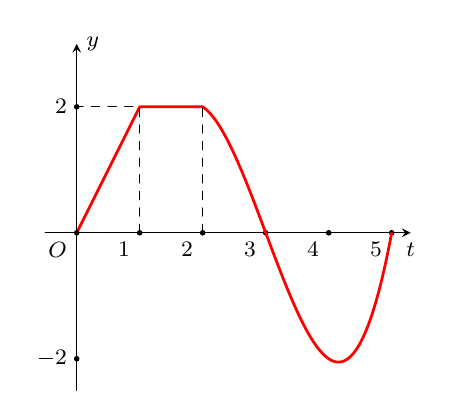
\begin{tikzpicture}[font=\footnotesize, line join=round, line cap=round, >=stealth, scale = 0.8]
			\draw[->] (-.5,0) --(0,0) node[below left]{$O$}--(5.3,0) node[below]{$t$};
			\draw[->] (0,-2.5) --(0,3) node[right]{$y$};
			\draw[fill = black] (1,0) node[below left]{$1$} circle (1pt) (2,0) node[below left]{$2$} circle (1pt) (3,0) node[below left]{$3$} circle (1pt) (4,0) node[below left]{$4$} circle (1pt) (5,0) node[below left]{$5$} circle (1pt);
			\draw[fill = black] (0,2) node[left]{$2$} circle (1pt) (0,-2) node[left] {$-2$} circle (1pt);
			\draw[line width = 1pt, red] (0,0)--(1,2)--(2,2);
			\draw[fill = black] (0,0) circle (1pt);
			\draw[line width = 1pt, red] 
			plot[domain=2:5, samples=100] (\x, {2/3*((\x)^3-9*(\x)^2+23*(\x)-15)});
			\draw[dashed] (1,0)--(1,2)--(0,2) (2,0)--(2,2);
		\end{tikzpicture}
	\end{center}
	Các mệnh đề sau đây đúng hay sai?
	\choiceTF
	{\True Diện tích hình phẳng được giới hạn các đồ thị hàm số $y=f(t)$, trục $O t$ và hai đường thẳng $t=0$; $t=1$ là $S=\dfrac{1}{2} \displaystyle\int\limits_{0}^{1} t \mathrm{\,d} t=\dfrac{1}{4}$}
	{\True Diện tích hình phẳng được giới hạn các đồ thị hàm số $y=f(t)$, trục $Ot$ và hai đường thẳng $t=1$; $t=2$ là $S=\displaystyle\int\limits_{1}^{2} 2 \mathrm{\,d}t=2$}
	{\True Tích phân $\displaystyle\int\limits_{2}^{3} f(x) \mathrm{\,d} x$ biểu thị cho phần diện tích của hình phẳng giới hạn các đồ thị hàm số $y=f(t)$, trục $O t$ và hai đường thẳng $t=2$; $ t=3$}
	{Tích phân $\displaystyle\int\limits_{3}^{5} f(x) \mathrm{\,d} x$ biểu thị cho phần diện tích của hình phẳng giới hạn các đồ thị hàm số $y=f(t)$, trục $O t$ và hai đường thẳng $t=3$; $ t=5$}
	\loigiai{
		\begin{itemchoice}
			\itemch Đúng. Vì đồ thị hàm số $y=f(t)$ trên đoạn $\left[0 ; 1\right]$ là $y=\dfrac{1}{2} t$. Do đó diện tích hình phẳng được giới hạn các đồ thị hàm số $y=f(t)$, trục $Ot$ và hai đường thẳng $t=0$; $t=1$ là $S=\dfrac{1}{2}\displaystyle\int\limits_{0}^{1} t \mathrm{\,d} t=\dfrac{1}{4}$.
			\itemch Đúng. Vì trên đoạn $ \left[1;2\right] $ đồ thị hàm số $y=f(t)=2$ nên hình phẳng được giới hạn bởi các đồ thị hàm số $ y=f(t) $, trục $O t$ và hai đường thẳng $t=1$; $t=2$ có diện tích là $S=\displaystyle\int\limits_{1}^{2} 2 \mathrm{\,d}t=2$.
			\itemch Đúng. Tích phân $\displaystyle\int\limits_{2}^{3} f(x) \mathrm{\,d} x=\displaystyle\int\limits_{2}^{3} f(t) \mathrm{\,d} t$ nên giá trị của tích phân $\displaystyle\int\limits_{2}^{3} f(t) \mathrm{\,d} t$ là diện tích của hình phẳng giới hạn các đồ thị hàm số $y=f(t)$, trục $Ot$ và hai đường thẳng $t=2$; $t=3$.
			\itemch Sai. Tích phân $\displaystyle\int\limits_{3}^{5} f(x) \mathrm{\,d} x=\displaystyle\int\limits_{3}^{5} f(t) \mathrm{\,d} t$.\\
			Diện tích hình phẳng được giới hạn các đồ thị hàm số $y=f(t)$, trục $O t$ và hai đường thẳng $t=3$; $t=5$ là $S=\displaystyle\int\limits_{3}^{5} \left|f(t)\right| \mathrm{\,d} t$.
		\end{itemchoice}
	}
\end{ex}

\Closesolutionfile{ans}
% \indapan{3}{ans/ans-2-C4B3CD1_10-19-DS}

\Opensolutionfile{ans}[ans/ans-C4B3CD1_20-26-KQ]
%\TNSA
%Câu 36

\begin{ex}%[2D4N3-1]
	Tính diện tích hình phẳng được tô màu trong hình bên dưới.
	\begin{center}
		\begin{tikzpicture}[font=\footnotesize, line join=round, line cap=round, >=stealth, scale = 1]
			\draw[->] (-.5,0) --(0,0) node[below left]{$O$}--(2.7,0) node[below]{$x$};
			\draw[->] (0,-.5) --(0,2.5) node[right]{$y$};
			\draw[fill = black] (1,0) node[below]{$1$} circle (1pt) (2,0) node[below]{$2$} circle (1pt);
			\draw[fill = black] (0,1) node[left]{$1$} circle (1pt)  (0,2) node[left]{$2$} circle (1pt);
			\draw[fill = black] (0,0) circle (1pt);
			\draw[dashed](0,2)--(2,2);
			\draw[line width =0.5 pt] (0,1) node[above right]{$ A $}--(2,2) node[above ]{$ B $}--(2,0) node[above right]{$ C $};
			\fill[pattern=north west lines] (0,1)--(2,2)--(2,0)--(0,0)--cycle;
			
		\end{tikzpicture}
	\end{center}
	\shortans{$ 3 $}
	\loigiai{
		\textbf{Cách 1:} Hình phẳng đã cho là hình thang vuông $ AOCB $, vuông tại $ A $, $ O $. Ta có
		$$ S=\dfrac{\left(AO+BC\right)\cdot OC}{2}=3.$$
		\textbf{Cách 2:} Đường thẳng $ AB $ đi qua hai điểm $ A\left(0;1\right) $ và $ B\left(2;2\right) $ nên đường thẳng $ AB $ có phương trình là $ y=\dfrac{1}{2}x+1 $.\\
		Hình phẳng đã cho giới hạn bởi đường thẳng $ y=\dfrac{1}{2}x+1 $, $ y=0 $, $ x=0 $, $ x=2 $ nên diện tích của hình phẳng là $ S=\displaystyle\int\limits_0^2 \left|\dfrac{1}{2}x+1 \right| \mathrm{\,d} x=3$.
	}
\end{ex}

%Câu 37
\begin{ex}%[2D4H3-1]
	Biết diện tích phần hình phẳng gạch chéo trong hình vẽ bên có diện tích là $ \dfrac{a}{b} $ với $ a$, $b \in \mathbb{Z} $ và phân số $ \dfrac{a}{b} $ tối giản. Tính tổng $ a+b $.
	\begin{center}
		\begin{tikzpicture}[font=\footnotesize, line join=round, line cap=round, >=stealth, scale = 1]
			\draw[->] (-.5,0) --(0,0) node[above left]{$O$}--(4.5,0) node[below]{$x$};
			\draw[->] (0,-.5) --(0,3.8) node[right]{$y$};
			\draw[fill = black] (1,0) node[below]{$1$} circle (1pt) (2,0) node[below]{$2$} circle (1pt);
			\draw[fill = black] (0,1) node[left]{$1$} circle (1pt)  (0,2) node[left]{$2$} circle (1pt);
			\draw[fill = black] (0,0) circle (1pt);
			\draw[dashed](1,0)--(1,1)--(0,1);
			\draw[line width = 0.5pt] plot[domain=0.2:3.8, samples=100] (\x, {((\x)-2)^2});
			\draw[line width = 0.5pt] plot[domain=-.5:3.6, samples=100] (\x, {(\x)});
			\fill[pattern=north west lines] (0,0)-- plot[domain=0:1](\x,{(\x)}) --(1,1)-- plot[domain=1:2](\x, {((\x)-2)^2}) --(2,0) --cycle;
			\draw (1.5,1.5)node[above,rotate=45]{\scriptsize $ y=x $};
			\draw (3.8,1)node[below]{\scriptsize $ y=\left(x-2\right)^2 $};
		\end{tikzpicture}
	\end{center}
	\shortans{$ 11 $}
	\loigiai{
		Dựa vào đồ thị, diện tích hình phẳng cần tìm là
		
		$S = \displaystyle\int\limits_{0}^{1} x \mathrm{\,d} x + \displaystyle\int\limits_{1}^{2}(x-2)^{2} \mathrm{\,d} x = \dfrac{1}{2} + \dfrac{1}{3} = \dfrac{5}{6}$.\\
		Vậy $ a=5 $; $ b=6 $ và $ a+b=11 $.
		
	}
\end{ex}

%Câu 38
\begin{ex}%[2D4H3-1]
	Biết diện tích phần tam giác cong $ OAB $ trong hình vẽ bên có diện tích là $ \dfrac{a}{b} $ với $ a$, $b \in \mathbb{Z} $ và phân số $ \dfrac{a}{b} $ tối giản. Tính hiệu $ b-a $.
	\begin{center}
		\begin{tikzpicture}[font=\footnotesize, line join=round, line cap=round, >=stealth, scale = 1]
			\draw[->] (-1.5,0) --(0,0) node[above left]{$O$}--(5.3,0) node[below]{$x$};
			\draw[->] (0,-1.5) --(0,4.5) node[right]{$y$};
			\foreach \x in {-1,1,2,3,4,5} \draw[fill] (\x,0) circle (1pt) node [below] { $\x$};
			\foreach \y in {-1,1,2,3,4} \draw[fill] (0,\y) circle (1pt) node [left] { $\y$};
			\draw[fill = red] (0,0) circle (1.2pt);
			\draw[line width = 0.5pt] plot[domain=-1.1:1.6, samples=100] (\x, {(\x)^3});
			\draw[line width = 0.5pt] plot[domain=-.1:4.1, samples=100] (\x, {((\x)-2)^2});
			\draw (1.5,3.5)node[left]{\scriptsize $ y=x^3 $};
			\draw (4,4.2)node[right]{\scriptsize $ y=x^2-4x+4 $};
			\draw[fill=red] (1,1) node[right]{$ A $} circle (1pt) (2,0) node[above right]{$ B $} circle (1pt);
		\end{tikzpicture}
	\end{center}
	\shortans{$ 5 $}
	\loigiai{
		Dựa vào hình vẽ ta thấy hình phẳng cần tính diện tích gồm 2 phần.\\
		Phần 1: Hình phẳng giới hạn bởi đồ thị hàm số $y=x^3$, trục $Ox$, $x=0$, $x=1$.\\
		Phần 2: Hình phẳng giới hạn bởi đồ thị hàm số $y=x^2-4 x+4$, trục $O x$, $x=1$, $x=2$.\\
		Do đó diện tích cần tính là 
		
		$S=\displaystyle\int\limits_{0}^{1}\left|x^3\right| \mathrm{\,d} x+\displaystyle\int\limits_{1}^{2}\left|x^2-4 x+4\right| \mathrm{\,d} x = \displaystyle\int\limits_{0}^{1} x^3 \mathrm{\,d} x + \displaystyle\int\limits_{1}^{2}\left(x^2-4 x+4\right) \mathrm{\,d} x = \dfrac{7}{12}$.\\
		Vậy $ a=7 $, $ b=12 $ và $ b-a=5 $.
	}
\end{ex}

%Câu 39
\begin{ex}%[2D4H3-1]
	Hình vuông $OABC$ có cạnh bằng $4$ được chia thành hai phần bởi đường cong $(C)$ có phương trình $y=\dfrac{1}{4} x^{2}$. Gọi $S_2$, $S_2$ lần lượt là diện tích của phần không tô màu và phần tô màu như hình vẽ bên dưới. Tỉ số $\dfrac{S_1}{S_2}$ bằng bao nhiêu?
	\begin{center}
		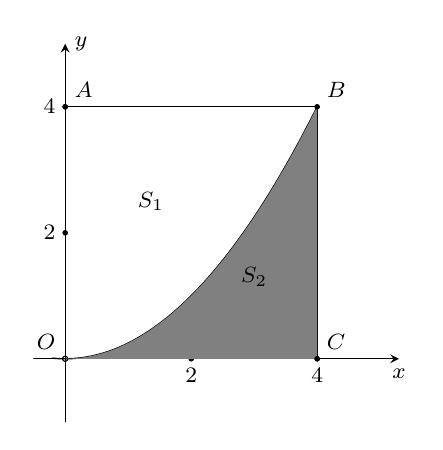
\begin{tikzpicture}[font=\footnotesize, line join=round, line cap=round, >=stealth, scale = 0.8]
			\draw[->] (-.5,0) --(0,0) node[above left]{$O$}--(5.3,0) node[below]{$x$};
			\draw[->] (0,-1) --(0,5) node[right]{$y$};
			\foreach \x in {2,4} \draw[fill] (\x,0) circle (1pt) node [below] { $\x$};
			\foreach \y in {2,4} \draw[fill] (0,\y) circle (1pt) node [left] { $\y$};
			\draw (0,0) circle (1.2pt);
			\draw[line width = 0.5pt] plot[domain=4:-.2, samples=100] (\x, {0.25*(\x)^2});
			\draw (4,0)--(4,4)--(0,4);
			\fill[gray] (0,0)-- plot[domain=0:4](\x,{0.25*(\x)^2})--(4,0)--cycle;
			\draw[fill=black] (0,4) node[above right]{$ A $} circle (1pt) (4,4) node[above right]{$ B $} circle (1pt) (4,0)node[above right]{$ C $} circle (1pt);
			\draw (1,2.5) node[right]{$ S_1 $} (3,1) node[above]{$ S_2 $};
		\end{tikzpicture}
	\end{center}
	\shortans{$ 2 $}
	\loigiai{Ta có diện tích hình vuông $O A B C$ là $ 16 $ và bằng $S_1+S_2$.\\
		Ta có $S_2=\displaystyle\int\limits_{0}^{4} \dfrac{1}{4} x^2 \mathrm{\,d} x =\left.\dfrac{x^3}{12}\right|_{0} ^{4}=\dfrac{16}{3} \Rightarrow \dfrac{S_1}{S_2}=\dfrac{16-S_2}{S_2}=\dfrac{16-\dfrac{16}{3}}{\dfrac{16}{3}}=2$.}
\end{ex}


%câu 40
\begin{ex}%[2D4V3-1]
	Cho hình thang cong $(H)$ giới hạn bởi các đường $y=\mathrm{e}^{x}$, $y=0$, $x=0$, $x=\ln 4$. Đường thẳng $x=k$, $(0<k<\ln 4)$ chia $(H)$ thành hai phần có diện tích là $S_1$ và $S_2$ như hình vẽ bên. Tìm $k$ để $S_1=2 S_2$ (làm tròn kết quả đến hàng phần chục).
	\begin{center}
		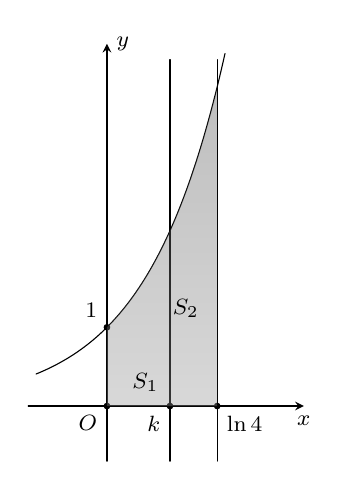
\begin{tikzpicture}[font=\footnotesize, line join=round, line cap=round, >=stealth, scale =1]
			\draw[->] (-1,0) --(0,0) node[below left]{$O$}--(2.5,0) node[below]{$x$};
			\draw[->] (0,-.7) --(0,4.6) node[right]{$y$};
			\draw[fill = black] (.8,0) node[below left]{$k$} circle (1pt);
			\draw[fill = black] (1.4,0) node[below right]{$\ln 4$} circle (1pt);
			\draw[fill = black] (0,1) node[above left]{$1$} circle (1pt);
			\draw[fill = black] (0,0) circle (1pt);
			\draw (.8,-.7)--(.8,4.4) (1.4,-.7)--(1.4,4.4);
			\draw [samples=100, domain=-.9:1.5] plot (\x, {e^(\x)});
			\fill[color=gray!10!black,shading=axis,opacity=0.2] (0,0) -- plot[smooth,samples=100,domain=0:1.4] (\x, {e^(\x)}) -- (1.4,0) -- cycle;
			\draw (0.2,.3) node[right]{$ S_1 $} (1,1) node[above]{$ S_2 $};
		\end{tikzpicture}
	\end{center}
	\shortans{$1,1$}
	\loigiai{
		Diện tích hình thang cong $(H)$ giới hạn bởi các đường $y=\mathrm{e}^{x}$, $y=0$, $x=0$, $x=\ln 4$ là
		$$S=\displaystyle\int\limits_{0}^{\ln 4} \mathrm{e}^{x} \mathrm{\,d} x = \mathrm{e}^{x}\Bigg|_{0}^{\ln 4}=\mathrm{e}^{\ln 4}-\mathrm{e}^{0}=4-1=3.$$\\
		Ta có $S=S_1+S_2=S_1+\dfrac{1}{2} S_1=\dfrac{3}{2} S_1$. Suy ra $S_1=\dfrac{2 S}{3}=\dfrac{2 \cdot 3}{3}=2$.\\
		Vì $S_1$ là phần diện tích được giới hạn bởi các đường $y=\mathrm{e}^{x}$, $y=0$, $x=0$, $x=k$ nên\\
		$
		2=S_1=\displaystyle\int\limits_{0}^{k} \mathrm{e}^{x} \mathrm{\,d} x=\mathrm{e}^{x}\Bigg|_{0}^{k}=\mathrm{e}^{k}-\mathrm{e}^{0}=\mathrm{e}^{k}-1$.\\
		Do đó $\mathrm{e}^{k}=3 \Leftrightarrow k=\ln 3 \approx 1{,}1$.}
\end{ex}

%câu 41
% \begin{ex}%[2D4V3-1]
% 	Cho hình phẳng $(H)$ giới hạn bởi các đường $y=\left|x^{2}-1\right|$ và $y=k$, với $0<k<1$. Tìm $k$ để diện tích hình phẳng $(H)$ gấp hai lần diện tích hình phẳng được kẻ sọc ở hình vẽ bên (làm tròn kết quả đến hàng phần trăm).
% 	\begin{center}
% 		\begin{tikzpicture}[font=\footnotesize, line join=round, line cap=round, >=stealth, scale =1]
% 			\draw[->] (-2,0) --(0,0) node[below left]{$O$}--(2,0) node[below]{$x$};
% 			\draw[->] (0,-3) --(0,3.3) node[right]{$y$};
% 			\draw[fill = black] (1,0) node[below left]{$1$} circle (1pt);
% 			\draw[fill = black] (0,1) node[above left]{$1$} circle (1pt);
% 			\draw[fill = black] (0,0) circle (1pt);
% 			\draw (-2,.4)--(2,.4) node[above right]{$ y=k $};
% 			\draw [samples=100, domain=-1:1] plot (\x, {-(\x)^2+1});
% 			\draw [samples=100, domain=-1:-1.8] plot (\x, {(\x)^2-1});
% 			\draw [samples=100, domain=1:1.8] plot (\x, {(\x)^2-1});
% 			\draw[dashed,samples=100,domain=-1:-1.8] plot (\x, {-(\x)^2+1});
% 			\draw[dashed,samples=100,domain=1:1.8] plot (\x, {-(\x)^2+1});
% 			\fill[pattern=north west lines] (-.77,.4) -- plot[smooth,samples=100,domain=-.77:.77] (\x, {-(\x)^2+1}) -- (.77,.4) -- cycle;
			
% 		\end{tikzpicture}
% 	\end{center}
% 	\shortans{$ 0{,}59 $}
% 	\loigiai{\begin{center}
% 			\begin{tikzpicture}[font=\footnotesize, line join=round, line cap=round, >=stealth, scale =1]
% 				\draw[->] (-2,0) --(0,0) node[below left]{$O$}--(2,0) node[below]{$x$};
% 				\draw[->] (0,-3) --(0,3.3) node[right]{$y$};
% 				\draw[fill = black] (1,0) node[below left]{$1$} circle (1pt);
% 				\draw[fill = black] (0,1) node[above left]{$1$} circle (1pt);
% 				\draw[fill = black] (0,0) circle (1pt);
% 				\draw (-2,.4)--(2,.4) node[above right]{$ y=k $};
% 				\draw [samples=100, domain=-1:1] plot (\x, {-(\x)^2+1});
% 				\draw [samples=100, domain=-1:-1.8] plot (\x, {(\x)^2-1});
% 				\draw [samples=100, domain=1:1.8] plot (\x, {(\x)^2-1});
% 				\draw[dashed,samples=100,domain=-1:-1.8] plot (\x, {-(\x)^2+1});
% 				\draw[dashed,samples=100,domain=1:1.8] plot (\x, {-(\x)^2+1});
% 				\fill[pattern=dots] (0,.4) -- plot[smooth,samples=100,domain=0:.77] (\x, {-(\x)^2+1}) -- (.77,.4) -- cycle;
% 				\fill[pattern=north west lines] (.77,.4)--plot[smooth,samples=100,domain=.77:1] (\x, {-(\x)^2+1}) -- plot[smooth,samples=100,domain=1:1.18] (\x, {(\x)^2-1}) -- (1.18,.4) -- cycle;
% 				\draw (0.77,.4) node[above]{$ A $} circle (1pt) (1.18,.4) node[above right]{$ B $} circle (1pt);
% 			\end{tikzpicture}
% 		\end{center}
% 		Gọi $S$ là diện tích hình phẳng $(H)$. Lúc dó $S=2 S_1+2 S_2$, trong đó $S_1$ là diện tích phần chấm bi và $S_2$ là diện tích phần gạch sọc trong hình vẽ bên.\\
% 		Gọi $A$, $ B$ là các giao điếm có hoành độ dương của đường thẳng $y=k$ và đồ thị hàm số $y=\left|x^{2}-1\right|$, trong đó $A(\sqrt{1-k}; k)$ và $B(\sqrt{1+k}; k)$.\\
% 		Theo yêu cầu bài toán
% 		\begin{eqnarray*}
% 			& & S=2 \cdot 2 S_1 \\
% 			& \Leftrightarrow & S_1=S_2 \\
% 			& \Leftrightarrow &\displaystyle\int\limits_{0}^{\sqrt{1-k}} \left(1-x^{2}-k\right) \mathrm{\,d} x =\displaystyle\int\limits_{\sqrt{1-k}}^{1}\left(k-1+x^{2}\right) \mathrm{\,d} x+\displaystyle\int\limits_{1}^{\sqrt{1+k}}\left(k-x^{2}+1\right) \mathrm{\,d} x \\
% 			& \Leftrightarrow & (1-k) \sqrt{1-k}-\dfrac{1}{3}(1-k) \sqrt{1-k}=\dfrac{1}{3}-(1-k)-\dfrac{1}{3}(1-k) \sqrt{1-k}+(1-k) \sqrt{1-k}+(1+k) \sqrt{1+k}-\dfrac{1}{3}(1+k) \sqrt{1+k}-(1+k)+\dfrac{1}{3} \\
% 			& \Leftrightarrow &\dfrac{2}{3}(1+k) \sqrt{1+k}=\dfrac{4}{3} \\
% 			& \Leftrightarrow & (\sqrt{1+k})^{3}=2\\
% 			& \Leftrightarrow & k=\sqrt[3]{4}-1\approx 0{,}59.
% 	\end{eqnarray*}}
	
% \end{ex}
\Closesolutionfile{ans}
% \indapan{6}{ans/ans-C4B3CD1_20-26-KQ}